%%%%%%%%%%%%%%%%%%%%%%%%%%%%%%%%%%%%%%%%%%%%%%%%%%%%%%%%%%%%%%%%%%%%%%%%%%%%%%%%
%%%%%%%%%%%%%%%%%%%%%%%%%%%%%%%%%%%%%%%%%%%%%%%%%%%%%%%%%%%%%%%%%%%%%%%%%%%%%%%%
%%                                                                            %%
%% thesistemplate.tex version 4.21 (2026/02/19)                               %%
%% The LaTeX template file to be used with the aaltothesis.sty (version 4.21) %%
%% style file.                                                                %%
%% This package requires pdfx.sty v. 1.5.84 (2017/05/18) or newer.            %%
%%                                                                            %%
%% This is licensed under the terms of the MIT license below.                 %%
%%                                                                            %%
%% Written by Luis R.J. Costa.                                                %%
%% Currently developed at Teacher services, Learning Services of Aalto        %%
%% University by Luis R.J. Costa since May 2019.                              %%
%%                                                                            %%
%% Copyright 2017-2026 aaltothesis.cls by Luis R.J. Costa,                    %%
%% luis.costa@aalto.fi.                                                       %%
%% Copyright 2017-2018 Swedish translations in aaltothesis.cls by Elisabeth   %%
%% Nyberg and Henrik Wallén henrik.wallen@aalto.fi.                           %%
%% Copyright 2017-2018 Finnish documentation in the template opinnatepohja.tex%%
%% by Perttu Puska, perttu.puska@aalto.fi, and Luis R.J. Costa.               %%
%% Finnish documentation in the template opinnatepohja.tex translated from    %%
%% the English template documentation.                                        %%
%% Copyright 2026 English template thesistemplate.tex by Luis R.J. Costa,     %%
%% Maurice Forget, Henrik Wallén.                                             %%
%% Copyright 2018-2026 Swedish template avhandlingsmall.tex by Henrik Wallen. %%
%%                                                                            %%
%% Permission is hereby granted, free of charge, to any person obtaining a    %%
%% copy of this software and associated documentation files (the "Software"), %%
%% to deal in the Software without restriction, including without limitation  %%
%% the rights to use, copy, modify, merge, publish, distribute, sublicense,   %%
%% and/or sell copies of the Software, and to permit persons to whom the      %%
%% Software is furnished to do so, subject to the following conditions:       %%
%% The above copyright notice and this permission notice shall be included in %%
%% all copies or substantial portions of the Software.                        %%
%% THE SOFTWARE IS PROVIDED "AS IS", WITHOUT WARRANTY OF ANY KIND, EXPRESS OR %%
%% IMPLIED, INCLUDING BUT NOT LIMITED TO THE WARRANTIES OF MERCHANTABILITY,   %%
%% FITNESS FOR A PARTICULAR PURPOSE AND NONINFRINGEMENT. IN NO EVENT SHALL    %%
%% THE AUTHORS OR COPYRIGHT HOLDERS BE LIABLE FOR ANY CLAIM, DAMAGES OR OTHER %%
%% LIABILITY, WHETHER IN AN ACTION OF CONTRACT, TORT OR OTHERWISE, ARISING    %%
%% FROM, OUT OF OR IN CONNECTION WITH THE SOFTWARE OR THE USE OR OTHER        %%
%% DEALINGS IN THE SOFTWARE.                                                  %%
%%                                                                            %%
%%                                                                            %%
%%%%%%%%%%%%%%%%%%%%%%%%%%%%%%%%%%%%%%%%%%%%%%%%%%%%%%%%%%%%%%%%%%%%%%%%%%%%%%%%
%%                                                                            %%
%%                                                                            %%
%% An example for writting your thesis using LaTeX                            %%
%% Original version and development work by Luis Costa, changes to the text   %% 
%% in the Finnish template by Perttu Puska.                                   %%
%% Support for Swedish added 15092014                                         %%
%% PDF/A-b support added on 15092017                                          %%
%% PDF/A-2 support added on 24042018                                          %%
%% Layout design and typesettin changed 15072021                              %%
%%                                                                            %%
%% This example consists of the files                                         %%
%%       thesistemplate.tex (version 4.21) (for text in English)              %%
%%       opinnaytepohja.tex (version 4.21) (for text in Finnish)              %%
%%       avhandlingsmall.tex (version 2.1) (for text in Swedish)              %%
%%       thesistemplate_short.tex (version 4.21) (abridged for text in        %%
%%                                                English)                    %%
%%       aaltothesis.cls (version 4.21)                                       %%
%%       linediagram.pdf (graphics file)                                      %%
%%       curves.pdf      (graphics file)                                      %%
%%       ledspole.jpg    (graphics file)                                      %%
%%                                                                            %%
%%                                                                            %%
%% Typeset in Linux with                                                      %%
%% pdflatex: (recommended method)                                             %%
%%             $ pdflatex thesistemplate                                      %%
%%             $ pdflatex thesistemplate                                      %%
%%                                                                            %%
%%   The result is the file thesistemplate.pdf that is PDF/A compliant, if    %%
%%   you have chosen the proper \documenclass options (see comments below)    %%
%%   and your included graphics files have no problems.                       %%
%%                                                                            %%
%%                                                                            %%
%% Explanatory comments in this example begin with the characters %%, and     %%
%% changes that the user can make with the character %                        %%
%%                                                                            %%
%%%%%%%%%%%%%%%%%%%%%%%%%%%%%%%%%%%%%%%%%%%%%%%%%%%%%%%%%%%%%%%%%%%%%%%%%%%%%%%%
%%%%%%%%%%%%%%%%%%%%%%%%%%%%%%%%%%%%%%%%%%%%%%%%%%%%%%%%%%%%%%%%%%%%%%%%%%%%%%%%
%%
%% WHAT is PDF/A
%%
%% PDF/A is the ISO-standardized version of the pdf. The standard's goal is to
%% ensure that he file is reproducable even after a long time. PDF/A differs
%% from pdf in that it allows only those pdf features that support long-term
%% archiving of a file. For example, PDF/A requires that all used fonts are
%% embedded in the file, whereas a normal pdf can contain only a link to the
%% fonts in the system of the reader of the file. PDF/A also requires, among
%% other things, data on colour definition and the encryption used.
%% Currently three PDF/A standards exist:
%% PDF/A-1: based on PDF 1.4, standard ISO19005-1, published in 2005.
%%          Includes all the requirements essential for long-term archiving.
%% PDF/A-2: based on PDF 1.7, standard ISO19005-2, published in 2011.
%%          In addition to the above, it supports embedding of OpenType fonts,
%%          transparency in the colour definition and digital signatures.
%% PDF/A-3: based on PDF 1.7, standard ISO19005-3, published in 2012.
%%          Differs from the above only in that it allows embedding of files in
%%          any format (e.g., xml, csv, cad, spreadsheet or wordprocessing
%%          formats) into the pdf file.
%% PDF/A-4: based on PDF 2.0, standard ISO19005-4, published in November 2020.
%%
%% PDF/A-1 files are not necessarily PDF/A-2 -compatible and PDF/A-2 are not
%% necessarily PDF/A-1 -compatible.
%% Standards PDF/A-1, PDF/A-2 and PDF/A-3 have two levels:
%% b: (basic) requires that the visual appearance of the document is reliably
%%    reproduceable.
%% a (accessible) in addition to the b-level requirements, specifies how
%%   accessible the pdf file is to assistive software, say, for the physically
%%   impaired.
%% The PDF/A-4 standard does not have additional levels like in the earlier
%% standards.
%% For more details on PDF/A, see, e.g., 
%% https://www.loc.gov/preservation/digital/formats/fdd/fdd000318.shtml or
%% https://www.pdfa.org/resource/iso-19005-pdfa/
%%
%%
%% WHICH PDF/A standard should my thesis conform to?
%%
%% Either to the PDF/A-2b or the PDF/A-1b standard. If all the figures and
%% graphs used in thesis work do not require transparency features, use either
%% PDF/A-1b or PFDF/A-2b. If you have figures with transparency
%% characteristics, use the PDF/A-2b standard. However, drawing applications
%% often use the transparency parameter, setting it to zero, to specify opacity
%% and get the basic 2-D visualisation. As a result, validation of PDF/A-1b
%% will fail. Use PDF/A-2b if PDF/A-1b validation fails.
%% Do not use the PDF/A-3b standard for your thesis.
%% The font to be used are specified in this templatenand they should not be
%% changed. In addition to not adhering to Aalto's visual guidelines, you may
%% have difficulties in producing a PDF/A-compliant PDF.
%%
%%
%% Validate your PDF/A file at https://www.pdf-online.com/osa/validate.aspx
%%
%%
%% WHAT graphics format can I use to produce my PDF/A compliant file?
%%
%% When using pdflatex to compile your work, favour the use of pdf, but you can
%% use the jpg or png format especially for photographs. You will have PDF/A 
%% compliance problems with figures in pdf if the fonts are not embedded in the
%% pdf file.
%% If you choose to use latex to compile your work, the only acceptable file
%% format for your figure is eps. DO NOT use the ps format for your figures.
%%
%% USE one of the following three \documentclass set-ups:
%% * the first when using pdflatex to directly typeset your document in the
%%   chosen pdf/a format for online publishing (centred page layout),
%% * the second for one-sided printing your thesis with the layout (wide left 
%%   margin), or
%% * the third for two-sided printing.
%%
\documentclass[english, 12pt, a4paper, sci, utf8, a-2b, online]{aaltothesis}
%\documentclass[english, 12pt, a4paper, elec, utf8, a-2b, print]{aaltothesis}
%\documentclass[english, 12pt, a4paper, elec, utf8, a-2b, print, twoside]{aaltothesis}

%% Use the following options in the \documentclass macro above:
%% your school: arts, biz, chem, elec, eng, sci
%% the character encoding scheme used by your editor: utf8, latin1
%% thesis language: english, finnish, swedish
%% make an archiveable PDF/A-1b or PDF/A-2b compliant file: a-1b, a-2b
%%                    (with pdflatex, a normal pdf containing metadata is
%%                     produced without the a-*b option)
%% typset for online document or print on paper: online, print
%%        online: typeset in symmetric layout and blue hypertext for online
%%                publishing
%%        print: typeset in a symmetric layout and black hypertext for printing
%%               on paper
%%        twoside: two-sided printing (default is one-sided printing)
%%                 typeset in a wide margin on the binding side of the page and
%%                 black hypertext. Use with print only.
%%

%% FOR USERS OF AMS PACKAGES:
%% * newtxmath used in this template loads amsmath, so
%%   you needn't load it. If you want to use options in amsmath, load it here, 
%%   before \setupthesisfonts below to pass the options to amsmath.
%% * If you want to use amsthm, load it here before \setupthesisfonts to avoid
%%   a clash with newtxmath.
%% * If using amsmath with options and you want to use amsthm, load amsthms
%%   after amsmath, as described in the amsthm documentation.
%% * Don't use amsbsym or amsfonts. The symbols [and macros] there are defined in
%%   newtxmath and so clash if used.
%\usepackage[options]{amsmath}

\usepackage{amsmath}
%\usepackage{amsfonts}
%\usepackage{amssymb}
%\usepackage{graphicx}


%% DO NOT MOVE OR REMOVE \setupthesisfonts
\setupthesisfonts

%%
%% Add here the packges you need
%%
\usepackage[utf8]{inputenc}
\usepackage[T1]{fontenc}
%\usepackage[latin2]{inputenc}
%\usepackage{t1enc}
%\usepackage[english]{babel}
%\usepackage{anysize}
\usepackage{graphicx}
\usepackage{tikz}
\usepackage{algorithm}
\usepackage{algpseudocode}
\usepackage{epstopdf}
\usepackage{fancyhdr}
\usepackage{etoolbox}
%\usepackage {xcolor}  
\usepackage[table,xcdraw]{xcolor}
\usepackage{float} 
\usepackage{wrapfig}
\usepackage{url}
\usepackage{hyperref}
\usepackage{color}
\usepackage{tabularray}


%% For tables that span multiple pages; used to split a paraphrasing example in
%% the appendix. If you don't need it, remove it.
%\usepackage{longtable}

%% A package for generating Creative Commons copyright terms. If you don't use
%% the CC copyright terms, remove it, since otherwise undesired information may
%% be added to this document's metadata.
\usepackage[type={CC}, modifier={by-nc-sa}, version={4.0}]{doclicense}
%% Find below three examples for typesetting the CC license notice.

\definecolor{Gray}{rgb}{0.67,0.67,0.67}

\usepackage{ntheorem}
\theoremstyle{change}
\makeatletter
\theoremseparator{.}
\newtheoremstyle{theoremstyle}%
{\item[\hskip\labelsep\theorem@headerfont
            ##2.\ ##1\theorem@separator]}%
{\item[\hskip\labelsep\theorem@headerfont
            ##2.\ ##1\theorem@separator\ (##3)]}%
\theoremstyle{theoremstyle}
\newtheorem{theorem}{Theorem}[section]
\newtheorem{defi}[theorem]{Definiton}

%% Edit to conform to your degree programme
%% Capitalise the words in the name of the degree programme: it's a name
\degreeprogram{ICT Innovation}
%%

%% Your major
%%
\major{Data Science}
%%

%% Choose one of the three below
%%
%\univdegree{BSc}
\univdegree{MSc}
%\univdegree{Lic}
%%

%% Your name (self explanatory...)
%%
\thesisauthor{Bálint János Prágai}
%%

%% Your thesis title and possible subtitle comes here and possibly, again,
%% together with the Finnish or Swedish abstract. Do not hyphenate the title
%% (and subtitle), and avoid writing too long a title. Should LaTeX typeset a
%% long title (and/or subtitle) unsatisfactorily, you might have to force a
%% linebreak using the \\ control characters. In this case...
%% * Remember, the title should not be hyphenated!
%% * A possible 'and' in the title should not be the last word in the line; it
%%   begins the next line.
%% * Specify the title (and/or subtitle) again without the linebreak characters
%%   in the optional argument in box brackets. This is done because the title
%%   is part of the metadata in the pdf/a file, and the metadata cannot contain
%%   linebreaks.
%%
\thesistitle{Merkle Tree-based framework for verifiable, incentivized and privacy-preserving data contribution systems: A Proof-of-concept}
%\thesistitle[Title of the thesis]{Title of\\ the thesis}
%%
%% Either remove or leave \thesissubtitle{} empty if you don't use it
%%
%\thesissubtitle{A possible subtitle}
%\thesissubtitle[Subtitle of the thesis]{Subtitle of\\ the thesis}
%\thesissubtitle{}

%%
\place{Espoo}
%%

%% The date for the bachelor's thesis is the day it is presented
%%
\date{29 May 2026}
%%

%% Thesis supervisor
%% Note the "\" character in the title after the period and before the space
%% and the following character string.
%% This is because the period is not the end of a sentence after which a
%% slightly longer space follows, but what is desired is a regular interword
%% space.
%%
\supervisor{Assoc. Prof. Alexander Jung}
%%

%% Advisor(s)---two at the most---of the thesis. Check with your supervisor how
%% many official advisors you can have.
%%
\advisor{Attila Papp (PhD Student)}
\advisor{Johanna Viio Löfberg (MSc)}
%%

%% If you do your thesis work in a company or other institution, give the name
%% of the company or instution here. Otherwise, leave the macro empty, comment
%% it out, or remove it. This will remove this field from the abstract page.
%%
\collaborativepartner{Fixmeapp AB}
%%

%% Aaltologo: syntax:
%% \uselogo{?|!|'|aalto?|aalto!|aalto'|<empty>}
%% The logo language is set to be the same as the thesis language.
%%
%\uselogo{?}
\uselogo{!}
%\uselogo{'}
%\uselogo{aalto?}
%\uselogo{aalto!}
%\uselogo{aalto'}
%\uselogo{}
%%

%%%%%%%%%%%%%%%%%%               COPYRIGHT TEXT               %%%%%%%%%%%%%%%%%%
%%%%%%%%%%%%%%%%%%%%%%%%%%%%%%%%%%%%%%%%%%%%%%%%%%%%%%%%%%%%%%%%%%%%%%%%%%%%%%%%

%% Copyright of a work is with the creator/author of the work regardless of
%% whether the copyright mark is explicitly in the work or not. You may, if you
%% wish---we encourage you to do so---publish your work under a Creative
%% Commons license (see creativecommons.org), in which case the license text
%% must be visible in the work. Write here the copyright text you want using the
%% macro \copyrighttext, which writes the text into the metadata of the pdf file
%% as well.
%%
%% Syntax:
%% \copyrigthtext{metadata text}{text visible on the page}
%%
%% CHOOSE ONE OF THE COPYRIGHT NOTICE STYLES BELOW.
%% IF USING THE CC TERMS, CHOOSE THE LICENSE YOU WANT TO USE.
%% The different CC licenses are listed at 
%% https://creativecommons.org/about/cclicenses/.
%% If you use the icons from the doclicense.sty package, add the package above
%% (\usepackage{doclicense}).
%% IMPORTANT NOTE!! Manually write the CC text in the \copyrighttext metadata
%% text field.
%%
%% NOTE: In the macros below, the text written in the metadata must have a
%% \noexpand macro before the \copyright special character. When not in pdf/a
%% mode (i.e. a-1b or a-2b are not specified in \documentclass), two \noexpands
%% are required in the metadata text to correctly render the copyright mark in
%% the pdf metadata. In pdf/a mode one \noexpand suffices.
%%
%% EXAMPLE OF PLAIN COPYRIGHT TEXT
%% The macros \copyright and \year below must be separated by the \ character 
%% (space chacter) from the text that follows. The macros in the argument of the
%% \copyrighttext macro automatically insert the year and the author's name.
%% (Note! \ThesisAuthor is an internal macro of the aaltothesis.cls class file).
%%
%\copyrighttext{Copyright \noexpand\textcopyright\ \number\year\ \ThesisAuthor}
%{Copyright \textcopyright{} \number\year{} \ThesisAuthor}
%%
%% Of course, the same text could have simply been written as
%% \copyrighttext{Copyright \noexpand\copyright\ 2018 Eddie Engineer}
%% {Copyright \copyright{} 2022 Eddie Engineer}
%%
%% EXAMPLES OF CC LICENSE: different ways to display the same license
%% 1. A simple Creative Commons license text with a link to the copyright notice:
%\copyrighttext{\noexpand\textcopyright\ \number\year. This work is 
%	licensed under a CC BY-NC-SA 4.0 license.}{\textcopyright{} 
%	\number\year. This work is licensed under a 
%	\href{https://creativecommons.org/licenses/by-nc-nd/4.0/}{CC BY-NC-SA 4.0} 
%	license.}
%
%% To get the URL of the license of your choice, go to 
%% https://creativecommons.org/about/cclicenses/, click on the chosen license
%% you want to use, and copy-and-paste the URL in the macro \href above.
%%
%% 2. A short Creative Commons license text containing the respective CC icons
%% (requires the package doclicense.sty to be added in the preamble as done
%% above) and a link to the corresponding Creative Commons license webpage (see
%% the doclicense package documentation for other license icons):
%\copyrighttext{\noexpand\textcopyright\ \number\year. This work is licensed
%	under a CC BY-NC-SA 4.0 license.}{
%	\parbox{95mm}{\noindent\textcopyright\ \number\year. \doclicenseText} 
%	\hspace{1em}\parbox{35mm}{\doclicenseImage}
%}
%%
%% 3. An expanded Creative Commons license text containing the respective CC
%% icons text and as generated by the doclicense.sty package (the license is set
%% via package options in \usepackage[options]{doclicense} above; see the
%% doclicense package documentation for other license texts and icons):
\copyrighttext{\noexpand\textcopyright\ \number\year. This work is 
	licensed under a Creative Commons "Attribution-NonCommercial-ShareAlike 4.0 
	International" (BY-NC-SA 4.0) license.}{\noindent\textcopyright\ \number
	\year \ \doclicenseThis}
%%%%%%%%%%%%%%%%%%%%%%%%%%%%%%%%%%%%%%%%%%%%%%%%%%%%%%%%%%%%%%%%%%%%%%%%%%%%%%%%


%% The English abstract:
%% All the details (name, title, etc.) on the abstract page appear as specified
%% above.
%% Thesis keywords:
%% Note! The keywords are separated using the \spc macro.
%%
\keywords{Ethical data economy, Ethical data market, privacy-preserving data ontribution system, Merkle tree, Wibson protocol}
%%

%% The abstract text. This text in one paragraph is included in the metadata of
%% the pdf file as well as the abstract page. To have paragraphs in your
%% abstract rewrite it in the abstarct environment as described below.
%%
\thesisabstract{%
Data became an increasingly sought-after commodity with the growth of AI and Machine Learning models, yet the profits rarely go to the users, who produce the data. Researchers have called for more ethical, human-centric practices and have laid out some possible frameworks for an ethical data economy. The aim of this thesis was to create a contribution system that would work well in an ethical data market. Using Merkle trees, this contribution system keeps the identity and data of the users safe, while still holding up to the FACT principles best to its ability.
}

%% You can prevent LaTeX from writing into the xmpdata file (it contains all the 
%% metadata to be written into the pdf file) by setting the writexmpdata switch
%% to 'false'. This allows you to write the metadata in the correct format
%% directly into the file thesistemplate.xmpdata.
%\setboolean{writexmpdatafile}{false}


%% All that is printed on paper starts here
%%
\begin{document}

%% Create the coverpage
%%
\makecoverpage

%% Typeset the copyright text.
%% If you wish, you may leave out the copyright text from the human-readable
%% page of the pdf file. This may seem like a attractive idea for the printed
%% document especially if "Copyright (c) yyyy Eddie Engineer" is the only text
%% on the page. However, the recommendation is to print this copyright text.
%%
\makecopyrightpage

\clearpage
%% Note that when writing your thesis in English, place the English abstract
%% first followed by the possible Finnish or Swedish abstract.

%% Abstract text
%% All the details (name, title, etc.) on the abstract page appear as specified
%% above. Add your abstarct text with paragraphs here to have paragraphs in the
%% visible abstract page. Nonetheless, write the abstarct text without
%% paragraphs in the macro \thesismacro so that it is added to the metadata as
%% well.
%%
\begin{abstractpage}[english]
Data became an increasingly sought-after commodity with the growth of AI and Machine Learning models, yet the profits rarely go to the users, who produce the data. Researchers have called for more ethical, human-centric practices and have laid out some possible frameworks for an ethical data economy. The aim of this thesis was to create a contribution system that would work well in an ethical data market. Using Merkle trees, this contribution system keeps the identity and data of the users safe, while still holding up to the FACT principles best to its ability.
\end{abstractpage}

%% The text in the \thesisabstract macro is stored in the macro \abstractext, so
%% you can use the text metadata abstract directly as follows:
%%
%\begin{abstractpage}[english]
%	\abstracttext{}
%\end{abstractpage}

%% Force a new page so that the possible Finnish or Swedish abstract does not
%% begin on the same page
%%
\newpage


\dothesispagenumbering{}

%% Preface
%%
%% This section is optional. Remove it if you do not want a preface.
\mysection{Preface}
%\mysection{Esipuhe}
I would like to thank my two my supervisors for their guidance. I want to thank Carlos Sarraute for partially advising my thesis. I owe thanks to Johanna Viio Löfberg for advising my thesis in the remaining time and the Fixmeapp academic team for working with me and aiding each others' research.
Finally, I would like to thank my friends, family and especially my girlfriend for supporting me and for giving me the strength to finish this project in the short time that I had for this.

\vspace{5cm}
Otaniemi, 29 May 2026\\


%% Force a new page after the preface
%%
\newpage


%% Table of contents. 
%%
\thesistableofcontents

%% \clearpage is similar to \newpage, but it also flushes the floats (figures
%% and tables).
%%
\cleardoublepage

%% Text body begins.
%%
\section{Introduction}
\label{sec:intro}

%% Leave page number of the first page empty
%% 
\thispagestyle{empty}

Current versions of data privacy oftentimes are opt-out models, giving users little control over their own data. The data is instead controlled by profit oriented organizations, profiling customers, exploiting them and their information, while the user receives no benefit from it. Usually combined with corner cuttings on safety \cite{vagle2020cybersecurity}\cite{kopp2017cyber}\cite{zhang2023market}, this results in numerous cases of Personal Identifiable Information (PII) leaks \cite{dao2021alternative}, that gives way to third party bad actors to reach an exploitable audience \cite{langvardt2024media}\cite{cross2025examining}, who should have been safe otherwise.\\
Furthermore, \cite{chen2023studying} proved, that collecting all the information (via cookies or any other ways) is not an optimal practice and the surplus of data creates storage and analysis issues.
There is significant amount of academic work that suggest the existence of an opt-in solution to replace primarily cookies. Not only that, but also in a way that is human-centric and confines to ethical frameworks.
This thesis is proposing a contribution system for a data market that is built on the above mentioned values, for a booking service.
This solution is Merkle tree based, cryptographically secured system, that works in an ethical way (follows the FACT principles \cite{sohail2024data}).\\
This chapter will further delve into the problems with current systems for data handling and data selling. In chapter two I showcase relevant literature regarding ethical data economy principles and models, data marketplace definitions and finally Merkle tree concepts with a focus on the inspiring paper of this thesis, the WibsonTree / Wibson protocol. Chapter three defines the research questions and methodology, as well as presenting relevant business cases and decisions taken while designing the proof-of-concept (PoC). Chapter four showcases the resulting PoC and Chapter five discusses the effectiveness and viability of the results and possible future directions for the project. The source code for the project will be available at the end of the thesis in the Source-code section and the provided GitHub repository.

\subsection{Relevance and problem definition}
%[Same as in intro, but further detailed on ethicalties, examples from privacy policies, EU vs USA, cookies and web hooks/web beacons, inefficiency, data leaks and their dangers, avoidability]
Cookies and other third party services have given ways for companies to gather data for free using opaque, complex methods \cite{altaweel2015web}\cite{demir2022towards}\cite{narayanan2017princeton}\cite{veale2022adtech}. This means no return for the generator of the data (the person using the services that collect the data) to benefit of their own contribution. More over, data collected this way is provably not stored securely, giving way to misuse of information, often for nefarious purposes \cite{langvardt2024media}\cite{cross2025examining}.\\
This means that these practices are exploitative, not transparent, fail to preserve privacy and not even optimal in most cases. These aspects are in direct contrast with many ethical frameworks, for example FACT (fairness, accuracy, confidentiality, transparency) principles \cite{sohail2024data}. Decentralized solutions, like blockchains, partially fulfill ethical requirements \cite{sansone2023blockchain}, but due to computational and infrastructural requirements are unfit for some commercial uses, such as booking services like hairdressers or manicures. They are also decentralized solutions, meaning they are not fit for a one-company business case.\\
Academic research clearly calls for an ethical data economy \cite{koskinen2019if}\cite{koskinen2023ethical}\cite{rantanen2020ethical}\cite{rantanen2020humans}, but not many commercially viable solutions exist. Fixmeapp AB aims to design a data marketplace to address the problems above. For that it needs a contribution system that adheres to an ethical framework, like FACT, centralized, and rewards users for their data. This thesis addresses the gap with the contribution system that qualifies for these requirements and allows user contributions to be tracked in a way that makes it possible for users to be rewarded after transactions, while their data is protected. A PoC of the contribution system should be sufficient in showing the system's fitness to the task.

%% In a thesis, every section/chapter starts a new page, hence the \clearpage
\clearpage

\section{Literature review}
This thesis aims to create a framework for verifiable and incentivized data contribution system in privacy-preserving manner, to serve as a building block for an ethical data market, that can later serve as foundation for an ethical data economy. 

After describing the methodology used for reviewing pertinent past releases, this chapter introduces the relevant definitions and concepts starting with definitions in data marketplaces, data transactions and privacy.
The review follows with showcasing the findings from the keyword scanning of applicable terms.

\subsection{Review methodology}
To design a system, that can stand up to these standards properly, multiple search terms were examined for this literature review. First search terms is "ethical data economy". Exact keyphrase matching on Google scholar \cite{scholargoogle_ethicaldataeconomy2026} resulted in 26 papers found, that were published since 2016.
Using consensus.app \cite{consensus_ethicaldataeconomy2026} for extended keyphrase lookup, another 120 hits were found, making it altogether 146. After title relevance-screening, duplicate filtering and article access checks, only 39 articles remain. Abstract screening eliminated another 22, leaving us with 17.
The second search term is "merkle tree" AND "hash", where a similar technique, but only on consensus.app \cite{consensus_merkleandhash2026} resulted in ~5400 initial hits. After deduplication and keyword relevance filtering, the number of relevant articles decreased to 48, further decreasing to 10 with title filtering. Abstract filtering left us with 4 papers.


%consensus got 120 hits since 2016 (extended keyword search), google scholar found 26 since 2016 (exact keyword matching)
%google(19.03.2026.): https://scholar.google.com/scholar?q=%22ethical+data+economy%22&hl=hu&as_sdt=0%2C5&as_ylo=2016&as_yhi= 
%consensus.ai(19.03.2026.): https://consensus.app/search/ethical-data-economy/619aS1rJQoCezJx8dpjegQ/?utm_source=share&utm_medium=clipboard

\subsection{Ethical data economy}

Data is a 'hot commodity' as it keeps gaining significance in our current world and is a basis for an economical system that dictates our lives. The larger a Machine Learning model gets the more data they require for training, making new models harder and harder to 'feed'. This resulted in some practices, that not all found human-centric, so call for ethical and human-centric data collection and handling practices grows ever louder.
One of the primary concerns laid out in \cite{hyrynsalmi2023balancing} is the secondary data market, also known as data reselling. This is a problem concerning many data economy models and is the root cause of many transparency issues. Consequently, it is a highly researched topic, but the consensus at the time of writing this thesis is that software-only solutions cannot protect against that.\\
%- Secondary data market usage \cite{hyrynsalmi2023balancing} <-> a system that hides the data itself, not the user\\

A couple of sources agree (\cite{valli2024ethical}, \cite{mirishli2025ethical}) that data economies are an ever-evolving landscape and should be treated accordingly. There should be constant exploration on what is happening, how data is used, how is it gathered and legal (e.g data and privacy protection laws) and ethical frameworks should constantly be recalibrated/reconceptualized. Similarly, current consent models are insufficient; consent for data gathering should be informed and adaptive. The research done by \cite{valli2024ethical} points to possible further explorations of data modification to achieve at least some of these goals. These are adding noise to the data artificially, consider different sensitivity for different kinds of data (e.g. treat phone number and health record protection differently) and exploring the privacy and utility trade-off, meaning the more private your data is, the less useful it is for systems. There should be some sort of balancing between the two, so all parties involved benefit the most.\\
%- prioritise transparent user mechanisms; use of federated learning; continuous recalibration and exploration; gaps: consideration of data sensitivity; privacy and utility enhancement trade-offs; adding noise to data \cite{valli2024ethical}\\
%- insufficient consent models; adaptive consent, regular reconceptualization of data protection laws \cite{mirishli2025ethical}\\

These demands for more ethicality in how our data is handled did not start recently. Already back in 2018 there were demands formed on how data usage should benefit society. First, it should be clear who benefits from the data, all parties who do and, probably more importantly, who incurs the risk \cite{hand2018aspects}. This means knowing that in case of e.g a data leak, whose information is getting exposed and what kind of information (e-mail address of an individual leaking has less negative impacts compared to their social security number becoming public). The paper talks about how these thoughts motivated multiple organizations; The European Data Protection Supervisor (EDPS) places human dignity in the center, using it to balance out surveillance and asymmetry of power against the individual. The Data governance working group rather uses human flourishing as a 'guiding star'.  Meaning systems running on human created data, should be designed and governed in a way that it supports the well-being of humans (the ones creating the data). The author does warn, that ethics do differ region-to-region (for example different principles are considered ethical in UK than the EU  or the USA), so systems trying to conform to ethics should be aware of their 'audience'. The author also gives a checklist of what ethical data governance systems should consider. Later showcased works define and list better considerations for the scope of the thesis, so this list is not given here.\\
%- be clear about who benefits who and who incurs the risk; EDPS: human dignity; Data Governance Working Group: human flourishing; ethics are not universal (EU vs UK vs USA); harm: health detriment, financial loss, discrimination, (gives and ethical checklist) \cite{hand2018aspects}\\
Rantanen and Koskinen started publishing in similar topics to the previous in 2019. Koskinen identified a gap in humanistic approaches to data governance, as demand started rising for it, especially in the EU \cite{koskinen2019if}. They identified the need for commonly accepted ground rules, which would start with a fair governance system (preferably an international one), but that is out of the scope of this thesis. Rantanen took a more down-to-earth approach, as they surveyed people's demand and expectation from an ethical data economy \cite{rantanen2019towards}. They found that people expect a system like this to support their autonomy, protect their privacy, to be secure and transparent, trustworthy, benevolent and just. As a whole they want it to be beneficial both to them as individuals and the rest of society.
%- people find these important: support autonomy, protect privacy, security, transparency, trustworthy, benevolent and just; beneficial to both individuals and society \cite{rantanen2019towards}\\
%- rising demand for more humanistic approaches; already some steps, at least in Europe; need for commonly accepted ground rules; starting point is fair governance, out of scope for this thesis \cite{koskinen2019if}\\
A year later, when talking about and defining a human-centric data economy, Rantanen et al. split human values into 2 groups: intrinsic and instrumental \cite{rantanen2020ethical}. Autonomy, justice and security of data are intrinsic values, while they categorized transparency, honesty and supervision instrumental ones. While their results are not absolute, they argue that these values should be included in a data economy that includes and is sustained by humans. Things that humans value should be studied more (and so should ways on how this can be done). These claims need to gain more rigor with further research, but this paper defined a direction for a part of the studies on data economy ethicality up until now. 
%- autonomy, justice and security are intrinsic values to a data economy; transparency, honesty and supervision are instrumental ones; these values must be included in the human-centric data economy; gaps: how to study these, more and deeper studies on what we, humans value \cite{rantanen2020ethical}\\
In the same year they continued this study in \cite{rantanen2020humans} which was a study done on over 8000 people, 4792 of which gave answers allowing for deeper insight, the summary of which can be found in Table \ref{tab:european_demand_summary}. There are 2 key takeaways here; The most pressing (and important) demand seems to be transparency, as not only large percentage of the participants demanded it, but is also enables the fulfillment of other demands, such as true control over data, informedness, security, trust or being in general aware of benefits. The second takeaway is that participants wanted an active role in a data economy; They want to have control over their data, be aware of what is happening to it (who can see it, who buys/uses it), benefit from the usage of their data and even in some cases the ability to supervise this system. The authors correctly identified a gap in communication between stakeholders at the time leading to large part of the demands. 
%- n = 4792 participants (non-representative of subgroups); \ref{tab:european_demand_summary}; 2 key takeaways: transparency is a demand and an enabler for other demands (true control, informedness, security, trust, be aware of benefits); active role: control over own data, be aware of what is happening to said data, benefit from this, maybe supervision of the systems; big pitfall is communication \cite{rantanen2020humans}\\
In their last paper of that year \cite{rantanen2020respecting} they built on the  identified values of their previous research and concluded, that human empowerment comes through information control. This means people should be able to control information about themselves; both what is visible and how it can be traded. To enable this, the paper suggests a good first step to be extending governance bodies to build trust in the whole data economy (stakeholder network).\\  
%- builds on prev paper on values; empowerment through information control; extend governance bodies to build trust in the entire network \cite{rantanen2020respecting}\\
The conclusion to their research saga would be their paper in 2023 \cite{koskinen2023ethical}. Here they discuss, how the current data economy practices and models are not in line with values of individuals and how there is a rising demand (and need) for an approach that follows ethical guidelines. They identified GDPR and similar frameworks have taken good steps towards this, but the current status is not sufficient. A good data ecosystem requires constant communication between stakeholders (as seen in \cite{rantanen2020humans}) and also facilitates it. This communication should focus on the data (and strategies) shared between these stakeholders. This constant communication would also enable regular restructuring of the system with active actors, as have been identified as a need previously. Their main point can be summarized in their quote: "Individuals are bypassed in the current data economy, which is strongly based on collecting from them." To achieve this, they identified a couple of next steps: The analysis and rethinking of current communication practices between stakeholders of data economies, research new, proper ways of effective communication and how viable they are.\\
%- current data economy is not in line with values of individuals, a need for more ethicality has risen; GDPR and alikes has been taken as good steps, but not enough; a good ecosystem requires and facilitates constant stakeholder interaction (see: pages 8 figure of the article); focus on the data and strategies shared between ecosystem stakeholders; constant communication and potential restructuring with active actors; "individuals are bypassed in the current data economy, which is strongly based on collecting from them"; gap: current communication practices between stakeholders, proper way of this communication, viability \cite{koskinen2023ethical}\\

A different approach in values to Rantanen and Koskinen also emerged in 2019. Devitt et al. collected all together 15 goals/principles around 4 topics: community, rights, usability and politics \cite{devitt2019principles}. "Community" refers to the data subjects, who produce the personal data fueling the data economies; these economies should be for these subjects and preferably ran by them, including communal sharing of information and self-governance. The "Rights" topic explores how data collection should respect human rights, benefit humans and the natural world. "Usability" is about the processing of the data and what it needs to be processable; it should be fit for purpose and usable, collected in a consensual, fair and transparent manner. Data is dependent on context (this context should be accounted for) and with reasonable exceptions it should be available to the public, to be revisable and form a useful social capital. "Politics" show how data can empower democratic people; data empowered people should be able to challenge existing political and economic norms, so they can revise this and achieve better, more equal and secure democracy. This approach was not as deeply researched as the one shown in the previous works, it does, however, consider the usability and transparency of the data and the seeming contradiction between them.\\
%- 15 principles: community: orchestrated and mediated by and for data subjects, including communal sharing for community decision making and self-governance; rights: should be collected with respect to humans and their rights and the natural world; usability: usable and fit for purpose; consensual, fair and transparent and must respect interpersonal relationships, data is dependent on context and with reasonable exceptions should be open and published, revisable and form useful social capital; politics: reveals and challenges the existing political and economic order so that data empowered people can secure good democracy. \cite{devitt2019principles}\\

The work of these authors made others evaluate the situation and come up with models for ethical data economies, especially in the age of AI and exponentially growing data demands. 
Hajoary et al. addresses the gap between ethicality and data monetization combined with AI data consumption \cite{hajoary2023exploring}. They reviewed the relevant literature and found that while AI, data base, Machine Learning were popular (high number of published papers), Ethics, law, rights were less researched. In these they identified a human need of transparency for data collected from them. Finally they further reinforce the need for culturally and ethically sensitive data governance policies, mostly in the EU and USA.\\
%- data monetization and AI data consumption don't align with ethical theories, that concern them; theoretical, ethical and methodological advancements; keywords of ethic, law, right, database, ai were popular in publishing; transparency is a big takeaway in human needs; reinforced needs for culturally sensitive data governance policies (in EU and USA)\cite{hajoary2023exploring}\\

Moran approached the question from the Big Data side \cite{moran2022towards}; They identified a gap between tools available and Big Data. Currently the latter outclasses the former in most aspects, leading to a non-transparent, overly powerful tool. This means Big Data requires deeper contemplation and rethinking, possibly reimplementation. Big Data needs to be handled in a way, that it is in accordance with human autonomy, while avoiding the pitfall of overregulation and regulatory loopholes. The invasiveness and number of people affected suggests using group ethics as ethical framework for resolving some moral dilemmas regarding the topic. The article finally warns, that Big Data systems should be aware of these limitations and especially dilemmas when being designed and should hold up to ethical frameworks.\\
%- operational challenges: people to be trained on data; Big Data exceeds current tools in capabilities; services created on the search of information; Big Data requires deep contemplation; moral responsibility - implementation with accordance to human autonomy; fear/pitfall of regulatory loopholes and overregulation; resolving moral dilemmas; must be aware of these limitations, especially the dilemmas; invasiveness and number of people affected call for uses of group ethics\cite{moran2022towards}\\

Okorie et al. further reinforce the need for consent, transparency and privacy in ethical data economies \cite{okorie2024ethical}. Furthermore, they identified a need for adaptable and inclusive ethical frameworks. They reason that these frameworks are addressing the complexities in the data subjects are generating and whom are affected by the data. They conclude that integrating ethical considerations into every step along the way of creating data economies is necessary, also can be referred to as 'ethical by design'.\\
%- consent and privacy are foundational elements for this; need for adaptable and inclusive ethical frameworks to address complexities; transparency; integrating ethical considerations into each and every step is necessary \cite{okorie2024ethical}\\

Keymolen and Taylor suggest putting responsibility on regulators and data scientists alike \cite{keymolen2023data}. They call for new regulations not only for data handling, but for those who are handling it. They argue data scientists should be accountable (as on go through rigorous evaluations, independent political influences) as their work directly and indirectly affects the lives of large portion of the population. They reason, because of the magnitude of the impact data science and data driven businesses have on society, more ethical research and business practices should be enforced. (Significant impact on society includes education, social relations, news, buying habits, media.) Data ethics as is, is unfit for this, as complexity of data demands it having open definitions and somewhat lose rules. This allows for malevolence in the form of ethics washing, which is dangerous while the ethics washed systems can impact society in this serious of a manner. This means data ethics need a revisit and ethics washing should be avoided at all cost.\\
%- call for new regulations; responsible data scientists, accountable (rigorous evaluations), no political incentives; reinforcement on more ethical business practice and data handling demands; data science and data-driven business have ethically significant impact in society (education, social relations, news, propaganda, buying); data ethics has a lot of open and sucks at defining what is the right thing to do -> ethics washing is a real danger, should be avoided at all costs.\cite{keymolen2023data}

Somewhat connected, a study in 2024 proposed a framework integrating some previously mentioned results and demands \cite{von2024data}. The article proposes a definition of data sovereignty as "The capability of a natural person or legal entity for exclusive self-determination with regard to its economic data goods" and lists several aspects of it. They argue the essentialism of data sovereignty for trusted data sharing between individuals and organizations/legal entities. They conclude that this trust between the different parties is essential in order to enable effective innovation. \\
%- data sovereignty: The capability of a natural person or legal entity for exclusive self-determination with regard to its economic data goods (has 7 aspects and their relations); essential to guaranteeing trusted data sharing between individuals and organization of different parties to make innovation happen \cite{von2024data}\\

The paper by Sohail et al. offers a better designed solution. They identified issues relating to individuals' matters \cite{sohail2024data}. These being data protection, fairness, transparency, confidentiality, integrity and autonomy. There was a framework that was close to solving those at the time, FAIR (findable, accessible, interoperable, reusable). While it was adopted in some areas, for mass adaption FAIR or FAIR principles would require coordinated efforts from multiple stakeholders, involving governing forces like federal governments or even the EU. They suggest an improvement on the framework in the form of the FACT (fairness (not as previous), accuracy, confidentiality, transparency) principles. This was developed (and to some extent adopted) in the Netherlands. Their improvement to this framework is the use of something called an Open Personal Data Store (OpenPDS). This Open version of PDS over the regular is required, so that it aligns with general business interest of not making all data public. (Important to note, that the study also shows enterprises holding onto data for longer doesn't make service any better. transparent and trustworthy companies are more likely to get data.) PDS allows for both queries and answers to happen in an encoded way, hiding data. OpenPDS further demands users have increased control over when they share data (privacy preservation and choice control) and this is how this system is the best we have so far.
%- issues relate to individuals' data protection, fairness, transparency, confidentiality, integrity and autonomy; solution (best, so far): FAIR(findable, accessible, interoperable, reusable) acclaimed and adopted; to achieve FAIR data, coordinated efforts from multiple stakeholders is required; FACT(fairness (not as prev), accuracy, confidentiality, transparency) developed and somewhat used in the Netherlands; Enterprises holding onto data for longer doesn't make service any better. transparent and trustworthy companies are more likely to get data; FAIR and OpenPDS(personal data store) --  data availability is not company interest; PDS is queried in code and answers in code; OpenPDS demands users have increased control over when they share data (privacy preservation and choice control) \cite{sohail2024data}\\




\begin{table}[H]
\centering
\caption{Summary of the demands surveyed by Rantanen and Koskinen (cited from \cite{rantanen2020humans})}
\refstepcounter{table}

\begin{tblr}{
  row{1} = {t},
  row{2} = {t},
  row{3} = {t},
  row{4} = {t},
  hlines = {Gray},
  vline{2} = {-}{Gray},
  hline{2} = {-}{0.08em},
}
Theme                              & Demands for a fair data economy                                                                                                                                                                                                                                                                                                                                                                                                              \\
Control over data and data sharing & {\labelitemi\hspace{\dimexpr\labelsep+0.5\tabcolsep}Power over data sharing and content\\\labelitemi\hspace{\dimexpr\labelsep+0.5\tabcolsep}Preserving privacy\\\labelitemi\hspace{\dimexpr\labelsep+0.5\tabcolsep}Informed and dynamic consent\\\labelitemi\hspace{\dimexpr\labelsep+0.5\tabcolsep}Possibility to control the content (requires access)\\\labelitemi\hspace{\dimexpr\labelsep+0.5\tabcolsep}Easy-to-use control mechanisms} \\
Transparency and being informed    & {\labelitemi\hspace{\dimexpr\labelsep+0.5\tabcolsep}Transparency of processes\\\labelitemi\hspace{\dimexpr\labelsep+0.5\tabcolsep}Ability to see what is collected\\\labelitemi\hspace{\dimexpr\labelsep+0.5\tabcolsep}Comprehensible and on-going communication}                                                                                                                                                                            \\
Security                           & {\labelitemi\hspace{\dimexpr\labelsep+0.5\tabcolsep}Secure services\\\labelitemi\hspace{\dimexpr\labelsep+0.5\tabcolsep}Confidentiality, anonymity\\\labelitemi\hspace{\dimexpr\labelsep+0.5\tabcolsep}Transparent data management\\\labelitemi\hspace{\dimexpr\labelsep+0.5\tabcolsep}Better understanding of security}                                                                                                                     \\
Trust and fairness                 & {\labelitemi\hspace{\dimexpr\labelsep+0.5\tabcolsep}Trustworthiness of service providers\\\labelitemi\hspace{\dimexpr\labelsep+0.5\tabcolsep}Clear promises that are kept\\\labelitemi\hspace{\dimexpr\labelsep+0.5\tabcolsep}Fair treatment of all parties}                                                                                                                                                                                 \\
Compensation and benefits          & {\labelitemi\hspace{\dimexpr\labelsep+0.5\tabcolsep}Concrete benefits for disclosing data\\\labelitemi\hspace{\dimexpr\labelsep+0.5\tabcolsep}Common good\\\labelitemi\hspace{\dimexpr\labelsep+0.5\tabcolsep}Clear and honest communication about the~benefits}                                                                                                                                                                             \\
Supervision and rules              & {\labelitemi\hspace{\dimexpr\labelsep+0.5\tabcolsep}Rules and laws are obeyed\\\labelitemi\hspace{\dimexpr\labelsep+0.5\tabcolsep}Supervision of the system by an independent institution\\\labelitemi\hspace{\dimexpr\labelsep+0.5\tabcolsep}Sanctions if rules are broken}                                                                                                                                                                 \\
Negative attitudes                 & {\labelitemi\hspace{\dimexpr\labelsep+0.5\tabcolsep}Trust needs to be gained back\\\labelitemi\hspace{\dimexpr\labelsep+0.5\tabcolsep}More holistic approach than a label needed}                                                                                                                                                                                                                                                            
\end{tblr}
\label{tab:european_demand_summary}
\end{table}

\subsection{Data marketplaces}
Data is a relatively new commodity \cite{haav2014data}. This means, that data markets and marketplaces were emerging in the 2010s, but as data was an unconventional product, the terminology across data sales was not uniform. \cite{stahl2016classification} successfully identified this gap and created a terminology framework that follows traditional market definitions, while adapting it to computer science environment. The following terminological framework will be used throughout this thesis;
\begin{defi}
    Market is an economic structure, the abstract place of trade, that serves three functions: Institute, transaction and pricing mechanism. As an institution market is a framework of rules, that assigns roles to its actors, as well as expected behaviors and protocols. The market is made up from the transactions happening in it, so the market defines these transactions. They consist of four phases; (1) Information phase (actors get informed about exchange intentions (bids/offers)), (2) negotiation phase (actors negotiate the product, contract terms and price), (3) transaction phase (contracts are fulfilled), (4) after-sales phase (customer service) \cite{richter2002elektronische}. As pricing mechanism, the market leads the actions of buyers and sellers and signal the conditions of sale to other participants. These definitions apply to electronic markets and in them to data markets. These only deviate in implementation of the institutionality and pricing philosophy as transaction costs are low and they are highly accessible.
\end{defi}
\begin{defi}
    An electronic marketplace is the concrete virtual institution and place of exchange that brings together supply and demand and supports the trade between providers and customers, i.e., transferring the market function into an electronic infrastructure. Any type of business action on online platforms or any type of electronic venture falls into this dimension with no regard to whether they are based on competition or on collaboration.
\end{defi}
A data market and marketplace conform to the definitions above. Based on those \cite{stahl2016classification} define them in the following way:
\begin{defi}
    Data marketplace is an electronic marketplace, where:
    \begin{itemize}
        \item A provider's primary business model needs to be providing data and/or related services. 
        \item Data marketplace provider's need to offer an infrastructure that allows customers to upload, browse, download, buy and sell machine-readable data. (e.g. CSV, XML, JSON) The data have to be hosted by the providers and it needs to be clear whether the specific data come from the community or the operator.
    \end{itemize}
\end{defi}

Furthermore, Figure \ref{fig:data_market_hier} shows the hierarchical analysis of the model proposed in \cite{stahl2016classification}, out of which this system could be either categorized as buy-side system or a buy-side platform, as the product (data) supply is in the hands of the platform owner. Many users individually produce data, but the platform owner collects it and offers it to the numerous, outside buyers. This warrants buy-side system as a better description of marketplace of the two.

\begin{figure}[H]
    \centering
    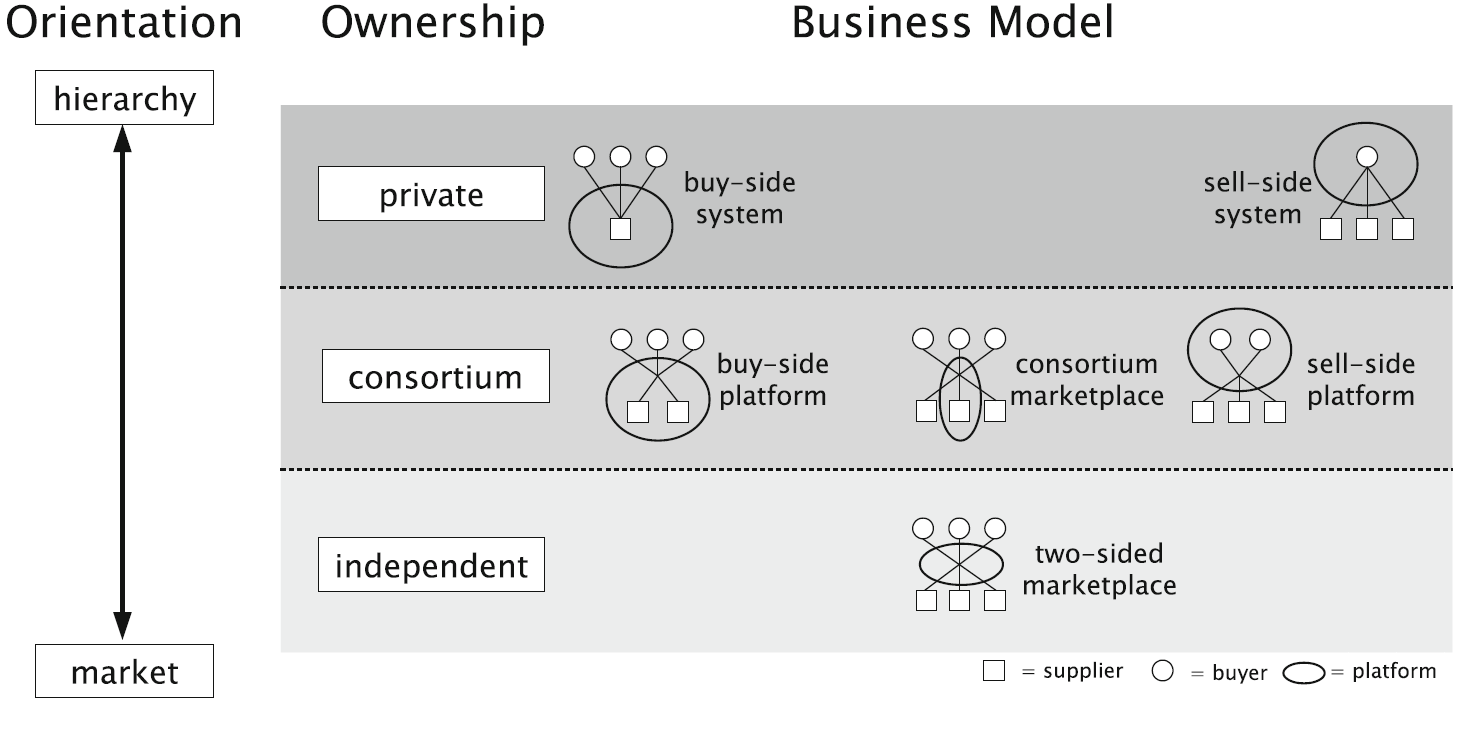
\includegraphics[width=1\linewidth]{images/datamarketdef.png}
    \caption{A model of electronic marketplaces discerning between three ownership types, cited from \cite{stahl2016classification}}
    \label{fig:data_market_hier}
\end{figure}



\subsection{WibsonTree and other Merkle tree concepts}

In their paper Liu et al. \cite{liu2021merkle} define the Merkle tree as "a kind of tree that obtains value of the parents and the root by combining each of its children and computing the hash value of the combination". (Picture in Fig. \ref{fig:merkle_base}) This is a technology implemented in blockchain technologies such as Bitcoin or Ethereum. The paper details 3 properties of the Merkle tree:
\begin{itemize}
    \item \textbf{Preimage resistance:} (or one-way hashing) is that for any fixed length hashed message $y$, it is computationally infeasible to figure out any specific $x$ input that produces that exact hash. Meaning, that the hashed message protects/masks the original information of said message, but still maps it with the fingerprint.
    \item \textbf{Second-preimage resistance:} A Merkle tree makes it computationally infeasible to find another message that has the same hash value as the original one. This protects against 'highjacking' or counterfeiting the original message.
    \item \textbf{Collision resistance:} For a Merkle tree (or its hash function) it is computationally infeasible to construct two different messages that produce the same hash value with the hash function. This enables Merkle trees to be used in data contribution systems, such as the one further detailed in \cite{futoransky2020wibsontree}.
\end{itemize}
As this concept is invented to work well on the blockchain, where every transaction is public and transparent, it solves the issue of efficient verification with only storing a header, which is useful for this thesis. The authors also make an important note, that these trees are not exclusively binary trees, but larger n-ary trees may require more resources for e.g. tree generation.\\
\begin{figure}[H]
    \centering
    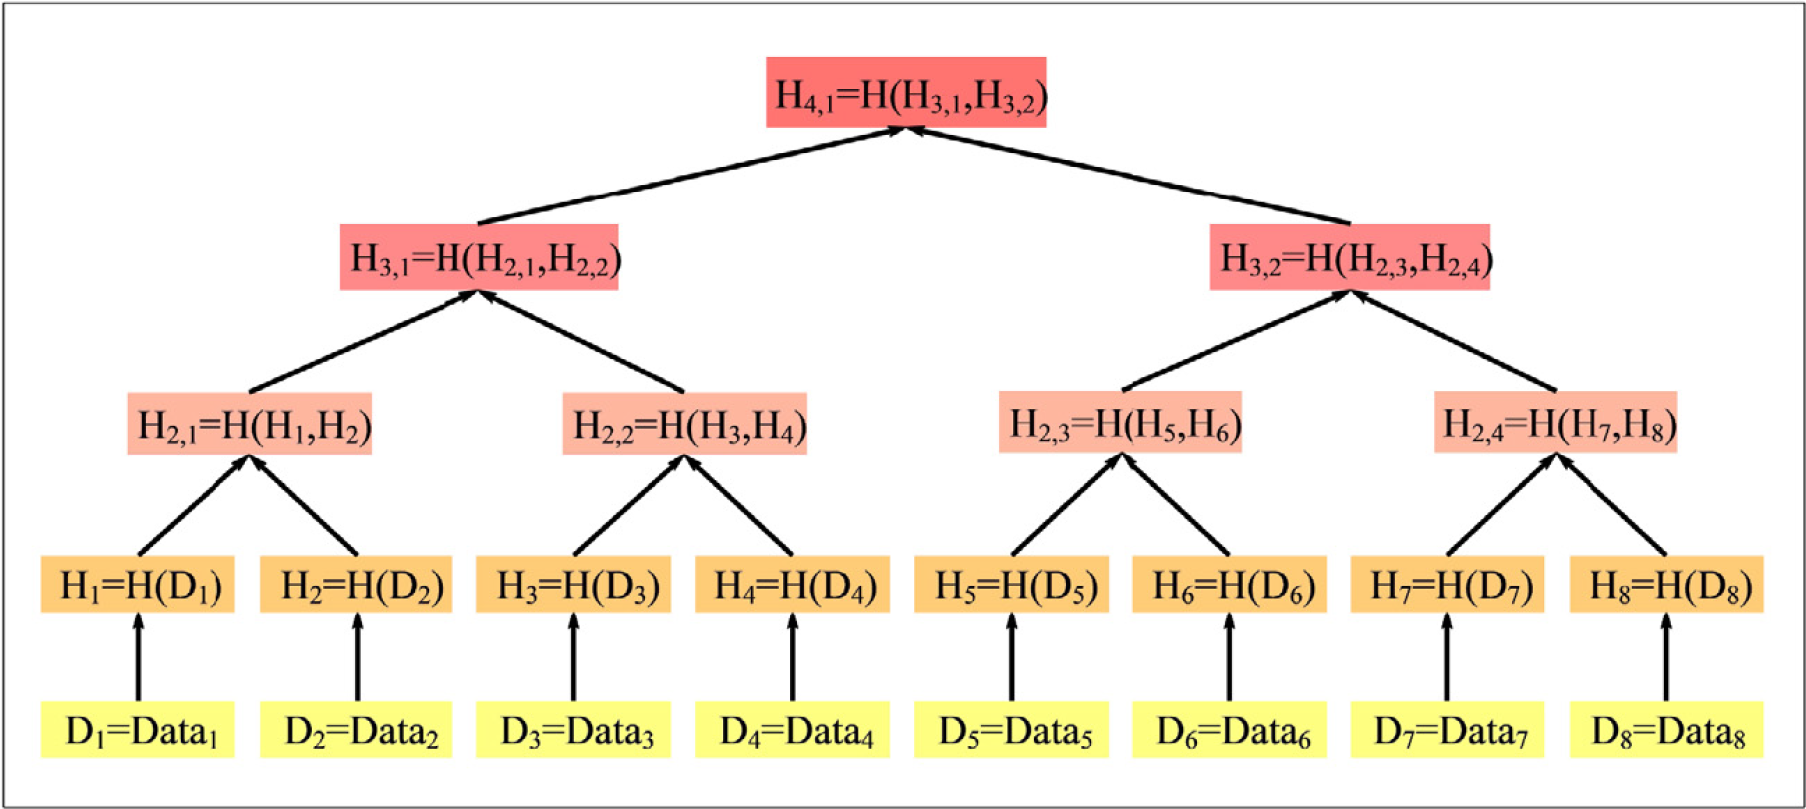
\includegraphics[width=1\linewidth]{images/merkle_tree.png}
    \caption{A Merkle tree created on 8 data points and with hash function $H(\cdot)$, cited from \cite{zhu2021improved}}
    \label{fig:merkle_base}
\end{figure}

In 2021 an improvement was proposed for Merkle trees encoding electronic medical records (EMR) \cite{zhu2021improved}. The authors propose an algorithm that turns the usual Merkle structure (pictured Fig. \ref{fig:merkle_base}) into a convolution structure using some Kernel (pictured Fig. \ref{fig:cnn_merkle}), inspired by convolutional neural networks. 

\begin{figure}[H]
    \centering
    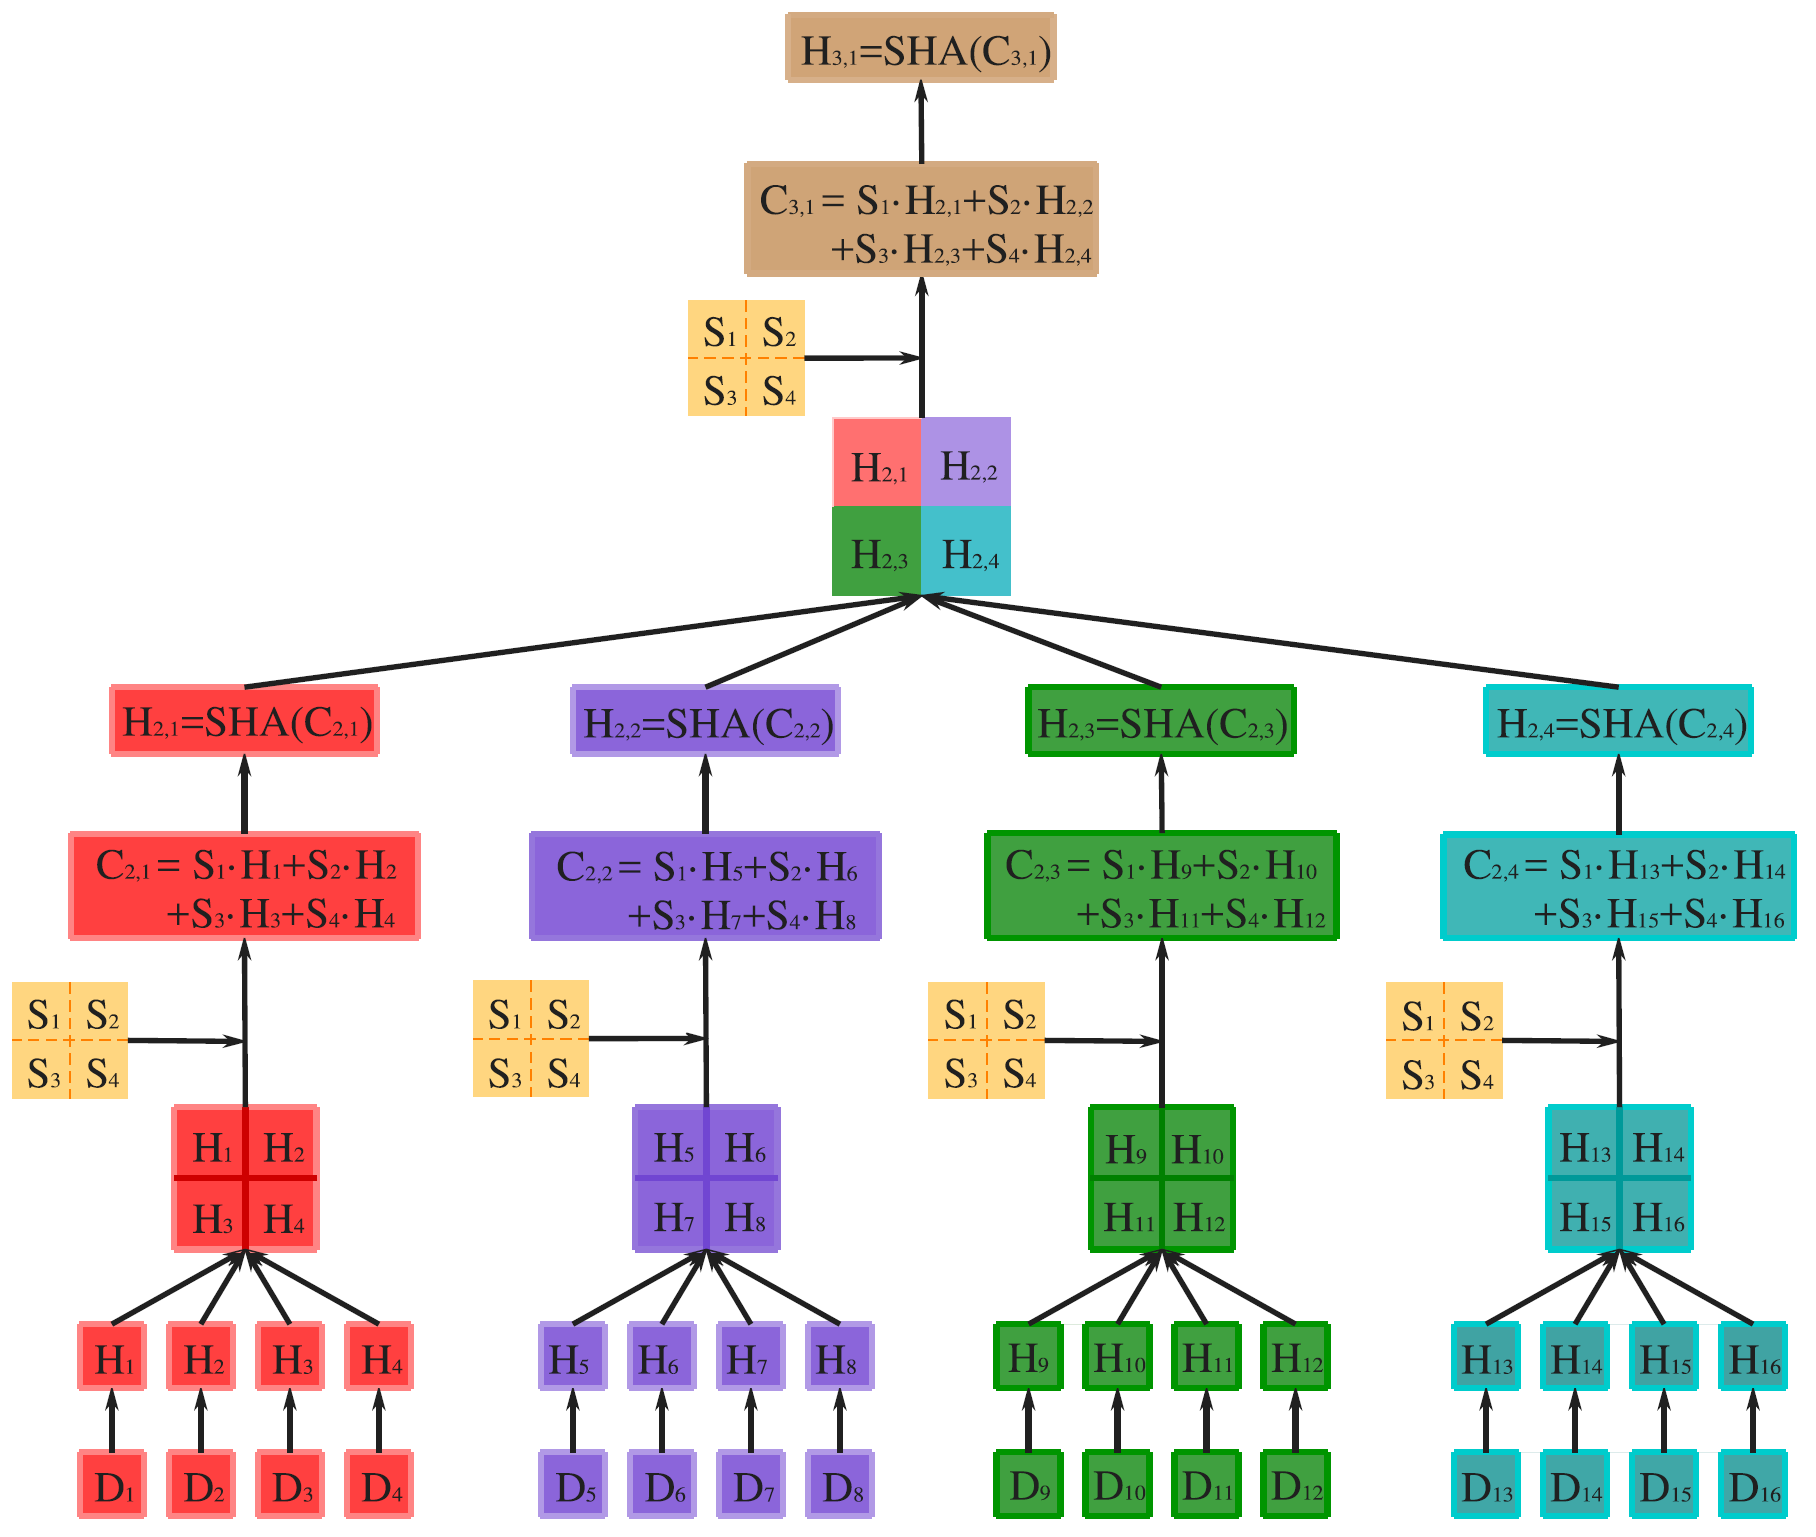
\includegraphics[width=1 \linewidth]{images/cnn_merkle.png}
    \caption{Layered Merkle tree with 16 data points, SHA256 hash function and $S$ convolution kernel, cited from \cite{zhu2021improved}}
    \label{fig:cnn_merkle}
\end{figure}

\noindent The example pictured requires the data to be able to be divided into 16 equal parts. This, however, is not a fixed number, it is dependent on the size of the kernel. Furthermore, noise can be added to 'fill out' the missing spots in the case of not enough data (e.g. 15 data blocks, one noise block in this case). This further increases privacy protection. Additionally, a significant speedup is proposed, as can be seen in Table \ref{tab:merkle_cnn_speed_diff}. Important to note, that this paper only considered this application in the EMR record and query application, it may not be guaranteed in different applications.



%\definecolor{SilverChalice}{rgb}{0.67,0.67,0.67}
\begin{table}
\centering
\caption{The difference between traditionaly k-ary merkle tree and the improved structure}
\label{tab:merkle_cnn_speed_diff}
\begin{tblr}{
  row{1} = {Gray,font=\bfseries},
  hlines,
  vlines,
}
Structure & Layer & Nodes                      & Hash calculations        \\
Original  & k*n+1 & $k^{2n+1}-1$               & $k^{2n}-1$               \\
Improved  & $n+1$ & $\frac{k^{2n+1}-1}{k^2-1}$ & $\frac{k^{2n}-1}{k^2-1}$ 
\end{tblr}
\end{table}

A significant potential upgrade to Merkle tree based systems are Recursive argument Merkle trees (Reckle trees) \cite{papamanthou2024reckle}. Papamanthou and their research group identified a gap in the calculations of proofs in Merkle trees, namely that they have to be fully recalculated, no matter the size of change in the data. Updatable batch proofs help blockchain systems efficiently compute and maintain proofs in a moving stream datablock setting. They propose and apply a technique called canonical hashing, allowing for batch proof updating in logarithmic time (though this requires sufficient parallelism, but provided that the speed would be batch size independent.) Canonical hashing is a recursive way to calculate a digest of a subset of leaves on the Merkle tree. This solution offers small memory footprint (112 KiB, independent of batch size), 10 to 15 times speed up on update time and 4.78 to 1485 times of speed up in verification under the right circumstances. While these results are likely to be well suited for industrial applications, they require too large resources for the proof of concept that is the scope of this thesis.\\
The paper by Liu et al. argues that the most popular form of hashing is Poseidon Hash for Merkle trees in the area of Zero-Knowledge Proofs (ZKP) \cite{liu2025acclmt}. Their identified research gap is how hardware acceleration can significantly speed up building Merkle trees with this type of hashing. While Poseidon is by default more expensive than traditional hashing (like SHA256) it scales better for certain hardware architecture and this is what this solution capitalizes on. Their proposed solution, AccIMT,  is a hardware-software combination that promises up to 1665 times speed up compared to other, software only solutions. Furthermore, it achieves 14.3 times speed and 14.8\% reduced area usage compared to previous state of the art in similar tech. The proposed experiment setup is optimized for blockchains and is at the time of writing unavailable for the purposes of thesis experimenting. This means while this solution is promising, it is both out of budget and out of scope for the thesis, while most likely promising a lucrative direction for further research.\\

The concept of WibsonTree \cite{futoransky2020wibsontree} introduces a data market model consisting of 3 types of actors:
\begin{itemize}
    \item The Buyer: Looking for data from individuals, that belong to a criteria (e.g. age: 25-30, sex: female). Only receives whether a Seller is matching this criteria, nothing else. Unaware if the same Seller is participating in multiple data transactions.
    \item The Seller: An individual, choosing to sell their own data, anonymously. The Seller has no information about other Sellers participating in a transaction. Under certain circumstances, also unaware of the Buyer's criteria.
    \item The Notary: They are the supervising actor of the marketplace. They are able to validate the precision and quality of the Sellers data. They should not be able to learn anything else about the Seller. They get compensated for their work. They need to have public identities and off-chain reputation. \cite{travizano2020wibson}
\end{itemize}
The Buyer specifies a criterion $X_0$. The Notary assigns a 'Match Criterion' function to each Seller $\mathcal{S}$, such that:
\begin{equation*}
    F_{\mathcal{S}}(X) \in \{true, false\};\\
    \forall X \neq X_0:
\end{equation*}
The Buyer does not learn the value of $F_{\mathcal{S}}(X)$. If a Seller matches criterion $X_0$, they reveal, that $F_{\mathcal{S}}(X_0) = true$, and the valuation is the same as the one signed by the Notary (Sign$_{Notary} (F_\mathcal{S}) = true$).

Additionally the Notaries have to name a 'verification price', that they charge for their work unrelated to the actual outcome of the transaction (it successfully happens or not). This prevents the Buyers from creating unlimited queries for free.
Using this function, the WibsonTree protocol builds a binary Merkle-tree-like structure with hashing, which allows for DAG and cryptographic proof creation. Proof is important, so the seller can be sufficiently identified on the blockchain and compensated after the data transaction successfully went through with the buyer.
Important to point out, while the design talks about, how the seller can withdraw consent to the data being sold, neither of the sources (\cite{futoransky2020wibsontree}, \cite{travizano2020wibson}) properly discuss exactly what happens and how in this given case.

\begin{figure}[H]
    \centering
    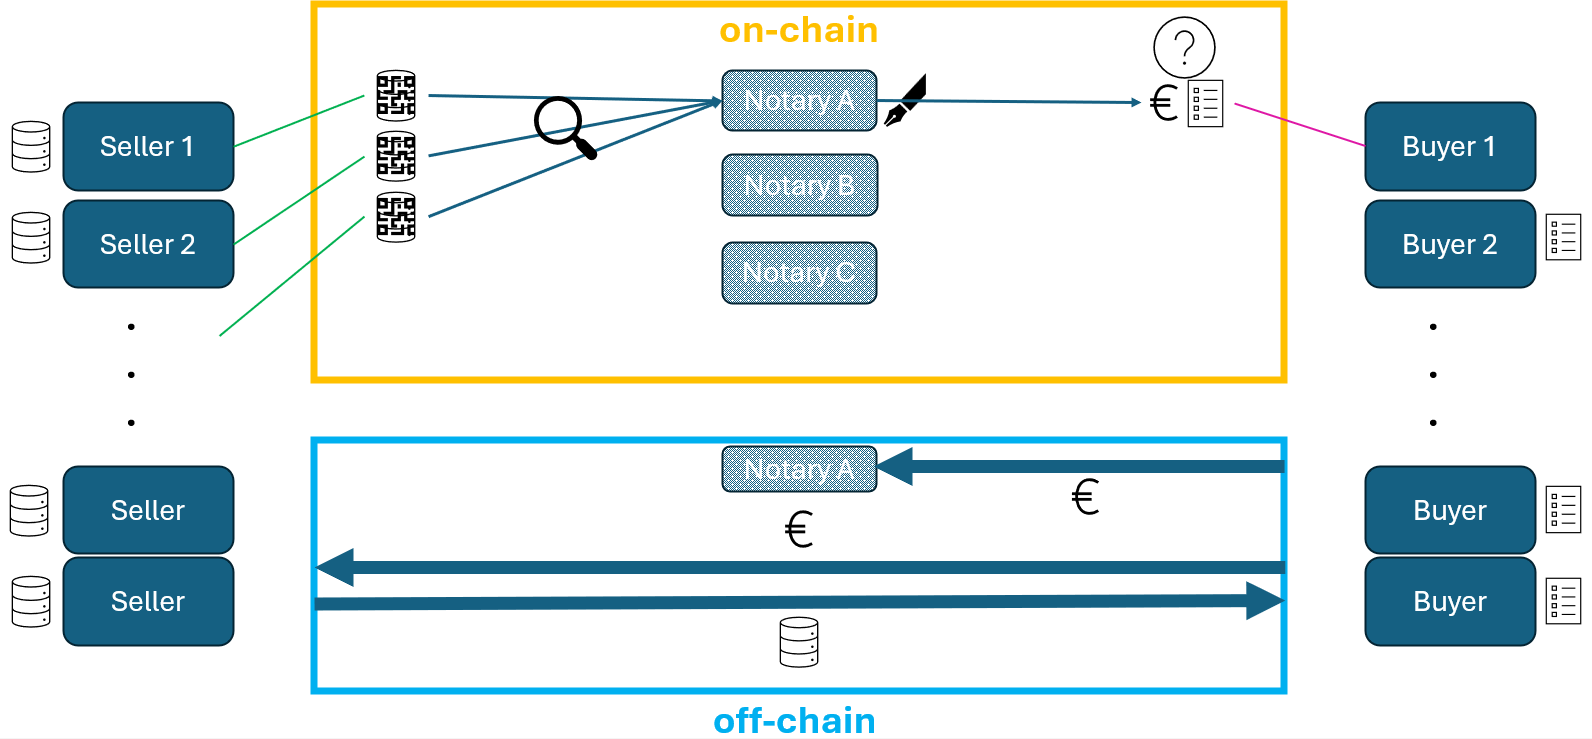
\includegraphics[width=1\linewidth]{images/wibson_tree.png}
    \caption{wibson protocol visualized}
    \label{fig:wib_tree_explain}
\end{figure}



This approach, however builds on raw data, that must be stored for the matching criterion to be calculated for every data request. In this form this can lead to PII leaks.
This warrants the need for a 2-step process, that anonymises the data first, then calculates the criterion.
The first step can be a good aggregation process, that generates a non-retraceable output. Then this can be 'fed' into the matching criterion and provide data to buyers this way.
Another good option is to collect already in a way that gives it some secrecy (e.g. age range, instead of age, geographical polygon instead of city). This, however is not possible with all kinds of information, those will need a case-by-case analysis.
Using the Wibson protocol, the seller can only get verification for the anonymised data. It's important to invent a way to be able for the proof to be connected back to the original Seller.

\clearpage

\section{Methodology and design}

This thesis is written in collaboration with the company Fixmeapp AB, that is a booking platform. The research questions, business cases and design decisions are defined in a way, to fulfill the needs for a booking platform, later a data market.

\subsection{Research problems}
Based on the results and the gaps of the literature review and the business request of the company (Namely to build a scalable data marketplace model, that is human-centric and ethical by design) the following research question are posed:\\
\textbf{RQ 1}: Can a contribution system designed for commercial use operate on at least the FACT principles? (Preferably conform to other ethical guidelines too)? \label{RQ1}\\
\textbf{RQ 2}: Is a 2-step data collection and criterion matching process sufficient to create a wibson-like protocol for ethical data economy model? \label{RQ2}\\
\textbf{RQ 3} :What proof can be generated, that still allows for the seller to be rewarded? \label{RQ3}% to be revised
\subsubsection{Metrics}
Research questions two and three are straightforward to answer and for the answer to be evaluated. Research question one does need some way of measuring success, however. The FACT principles are fairness, accuracy, confidentiality and transparency, all of which can be assigned a measure;
\begin{itemize}
    \item fairness: This thesis defines fairness for users as equality in contribution; meaning every user should be rewarded the same, on a per contribution basis. For this, the (discrete) Gini coefficient should be a good measure \cite{RePEc:oxp:obooks:9780198281931}: %Gini coefficient
    \begin{equation*}
     G = \frac{\Sigma^{n}_{i=1}\Sigma^{n}_{i=1}\| x_i-x_j \|}{2n(n-1)\overline{x}},   
    \end{equation*}
    where $n$ is the population, $x_i$ is the individual user's rewards and $\overline{x}$ is the average reward. A Gini coefficient of 0 reflects prefect equality between users, thus indicating a perfectly fair system, while a 1 means perfect inequality, meaning the system fails in upholding fairness.
    \item accuracy: As we don't have an objective constant truth, rather a case-by-case one, based on what criteria the Buyer needs matching. A "No-Truth" accuracy measure is the best choice for an accuracy metric. It works based on Expectation-Maximization and the estimation that maximizes this expectation is \cite{dawid1979maximum}: %dawid-skene, bc we have overlap and objective tasks: Dawid, A. P., & Skene, A. M. (1979). "Maximum Likelihood Estimation of Observer Error-Rates Using the EM Algorithm."
    \begin{equation*}
        \hat{\pi}^{(k)}_{jl} = \frac{\Sigma_i \mathbf{I}_{ij} n^{(k)}_{il}}{\Sigma_l \Sigma_i \mathbf{I}_{ij}n^{(k)}_{il}},   
    \end{equation*}
    where $\mathbf{I}_{ij}$ is an indicator function for buyer $i$, that is 1, when the criteria matches, 0 otherwise; $n^{(k)}_{il}$ is the number of attributes Buyer $k$ is trying to match.
    A more intuitive interpretation is 
    \begin{equation*}
        \hat{\pi}^{(k)}_{jl} = \frac{\text{\# times buyer $k$ records a non-match $l$ when looking for criteria $j$}}{\text{\# users seen by buyer $k$ matching criteria $j$}}
    \end{equation*}
    \item confidentiality: This thesis aims at creating a privacy preserving contribution system, so  confidentiality should come from this aspect. 
    Privacy preserving can be best measured with differential privacy that is defined by \cite{bugliesi2006automata}: %differential privacy 
    \begin{defi}
        A randomized function $\mathcal{K}$ gives $\epsilon$-differential privacy if $\forall$ datasets $D_1$ and $D_2$ differing on at most one entry, and all $S \subseteq \textit{Range}(K)$,
        \begin{equation*}
        \text{Pr}[\mathcal{K}(D_1) \in S] \leq exp(\epsilon) \times \text{Pr}[\mathcal{K}(D_2) \in S],
        \end{equation*}
    Where $Pr[.]$ is the privacy of the data.
    \end{defi}
    A low (close-to-0) $\epsilon$ value means high confidentiality, but low accuracy of the data, while a high one (5+) is low on confidentiality, but allows for better accuracy. This is a trade-off that has to be accounted for in design. The balance should be somewhere in the middle.
    
    \item transparency: This aspect is the hardest to measure and quantify. In their book  \cite{spagnuelo2016metrics} they managed to narrow down transparency to 8 metrics, accuracy being one of them. followed by currentness, conciseness, detailing, readability, availability, portability and effectiveness. As the scope of this thesis only has access to input data and no user or buyer interaction, (other than accuracy) the only realistic measures for this system is portability and effectiveness. %information symmetry ratio Turilli, M., & Floridi, L. (2009). "The Ethics of Information Transparency."
    \begin{itemize}
        \item Portability:
        \begin{equation*}
            P = \begin{cases}
                0, \text{if no information is available}\\
                0.2, \text{if available in any open format}\\
                0.4, \text{if available as structured data}\\
                0.6, \text{if available in non-proprietary format}\\
                0.8, \text{if uses URI}\\
                1, \text{if based on linked data}\\
            \end{cases}
        \end{equation*}
        Portability describes universality of the data: how easily it can be transferred and reused in other systems.
        \item Effectiveness:
        \begin{equation*}
            \mathcal{E} = \frac{\Sigma^{n_I}_{i=1}e_i}{\Sigma^{n_I}_{i=1}P^E_i} = 1 - \frac{\Sigma^{n_I}_{i=1}v_i}{\Sigma^{n_I}_{i=1}P^E_i},
        \end{equation*}
        where $n_I$ is the count of the output information upon query, $P^E_i = e_i + v_i$ is the number of questions appropriate to the effectiveness metric, divided into answered ($e_i$) and unanswered ($v_i$) questions.
        Effectiveness measures how good the output information is in answering questions such as: what? who? why? when? where?
    \end{itemize}
\end{itemize}

\subsubsection{Reformulation}
Now that we have defined the metrics for the FACT principles, \textbf{RQ 1} can be reformulated as follows:\\
\textbf{RQ 1r}\label{RQ1r}: Can a contribution system designed for commercial use achieve;
\begin{itemize}
    \item A Gini coefficient of $G < 0.5$
    \item Relatively high accuracy: $\hat{\pi}^{(k)}_{jl} \leq 1 \text{ , } \forall k$ and some criteria $j$
    \item Relatively high confidentiality: $\epsilon < 5$
    \item Portability of $0.4$ or higher
    \item Effectiveness $\mathcal{E} > 0.5$
\end{itemize}

\subsection{Methodology}
For this PoC to be formulated according to the three research questions, while still being a viable tool for the business setting laid out earlier, first possible business scenarios are laid out. After that the participants of the data market are defined, a decision is made between a decentralized and centralized model as well. Collecting, handling and storing the data is defined later in accordance with ethical and legal guidelines. Finally attack surfaces are laid out to show the possible internal and external threats and theoretical limitations of a framework like this. It is important to remember, while the design branches out and considers the whole of an ethical data market framework, the proof of concept and thus the scope of this thesis is limited to the contribution system of aforementioned data market.

\subsection{Possible business scenarios}\label{sec: business_scen}
Designing this framework requires it to function in certain ways, given predefined scenarios. Here we discuss three of the most likely cases that this system would be used in. We indicate in each case studied:
\begin{itemize}
    \item the stakeholders,
    \item the data collected and used,
    \item the sensitivity of different types of data,
    \item how this data is likely to be used and what the path of said data is,
    \item and finally analyze what critical functions the case requires and what are dangerous aspects, if any.
\end{itemize} 
The three scenarios analyzed here are a marketing campaign, a product development case and service provider self-improvement. The data involved in these cases is discussed in a manner that is realistic with regard of Fixmeapp business model as a booking company and what data could be realistically collected this way.

\subsubsection{Case 1: Marketing campaign}
In this first likely business case, the buyer would use the bought data for launching a marketing campaign. This can mean a marketing company or a marketing department of e.g. a skincare product company. The stakeholders in this case are; the Buyer (Marketing team/company), Governor (Fixmeapp), User(s). The data collected and stored about the user through bookings are manifold and most of it is quite valuable for the buyer in this case. The data in question in no particular order:
\begin{itemize}
    \item Geographical polygon data (same idea as can be seen with Wibson protocol \cite{futoransky2020wibsontree})
    \item Demographic data (age, biological sex OR gender, etc.)
    \item Booking history (with one particular company or all together, frequency can be inferred from these)
    \item (Based on booking history and geographical polygon, some sort of salary range can be inferred) % maybe? source?
\end{itemize}
Geographical polygon data and demographic data (for example; a male in their 30's, living in the general East-Uusimaa area) is not PII. Note, if the geographical polygon is not defined carefully/generally enough, it can lead to some sort of identification, combined with other data. Booking history with a particular partner in general is not sensitive, if stored correctly. (Bad example: male hair dying from blond to brunette, 10:30, [date], [saloon location]; Good example: male hair dying, [morning/afternoon/after work hours]). Data presented and purchased this way can be used to narrow down customer personas/profiles. These then can be used to design adverts or discount campaigns that accurately hit these customers, be it for retention or expanding client circles.\\
In this example the data would be generated by the users through booking, sent and stored by Fixmeapp and can be bought by the marketing departments/companies, that the users would be informed about. This process does not protect users against data reselling by the marketing companies, that could be for example a contractual obligation for the parties involved.\\

\subsubsection{Case 2: Product development}
In this business case the buyer acquires data in order to develop an existing or a new product, based on users of e.g. 
beautician services and the providers themselves. The stakeholders in this case are; the buyer (Product company), Governor (Fixmeapp), User(s) and Provider(s). The relevant data is much more narrow in this case, than the previous one, as much of the useful information, like what climate the product will be used in, has to be inferred from e.g. geographical polygons. Information that can prove useful:
\begin{itemize}
    \item Geographical polygon data. For inferring weather and humidity conditions, (tap) water quality.
    \item Demographic data (age, biological sex OR gender, etc.). This allows the producer to paint an accurate customer persona
    \item Booking history. For the same reasons as above. (Which saloons buy it, what kind of people want to use them)
    \item Allergies. There may be skin allergies affecting a larger portion of the customer population, that has to be taken into account when developing for example the recipe of a cream.
\end{itemize}
The first two bullet points still do not qualify as PII, given they are collected and stored in a reasonable manner. Booking history of a particular kind of provider (beautician - skin care, hairdresser - hair products, etc.) is in vast majority of the cases not enough to enable identification of any individual. Allergies, are however, different. This is health record data and should be stored and handled accordingly. \\
Similarly as the previous example, the data would be generated by the users through booking, sent and stored by Fixmeapp and be bought by companies, that the users would be informed about. This process does not protect users against data reselling by the marketing companies, that could be for example a contractual obligation for the parties involved. This second part is crucial in this case, as we are dealing with data qualifying as health record.\\

\subsubsection{Case 3: Service provider}
In this business case the service providers (at whom the users can book services through Fixmeapp's platform) want to improve the services they offer. They need data generated by the booking customers to see the pain points/shortcomings of their services (e.g. wrong opening hours, not offering a popular service).
The stakeholders in this case are; the buyer (Provider), Governor (Fixmeapp), User(s). The relevant data are things that are directly connected to the booking, circumstances of these and aftercare (e.g. ratings, what the user liked, what they did not like). More accurately:
\begin{itemize}
    \item Geographical polygon data. To understand the general range where they attract customers from and where they have competition because of this.
    \item Demographic data (age, biological sex OR gender, etc.). The sort of people booking their and similar services.
    \item Booking history. How often customers return, how often they go to competition for similar services, potentially what sort of other services they book together with the services provided by the provider.
    \item Ratings and complaint data. Crucial for identifying customer needs and pain points.
    \item (Based on booking history and geographical polygon, some sort of salary range can be inferred. This can help with pricing strategies.)
\end{itemize}
Just as with the other two examples, the first two points should not be able to be used for identification of a person. Combined with booking information, these all together should still not be enough to identify a person. Information acquired this way about competition should also not conflict with existing legal frameworks. (Prices, services available, products used are types of information, that a throughout competition analysis could reveal.) All listed data can be used to define competitive pricing and cater to a more optimized audience. The path of the data should be traceable throughout its journey, however an identical problem to the previous two cases arises; there is no way to guarantee protection against reselling the data.
All the business cases feature problems with secondary data markets or data reselling. This will be addressed later in this chapter, under Section \ref{sec:attack_surf}.

\subsection{Design decisions}
A data contribution system like this naturally poses a series of design questions. Firstly, while the solution is mostly based on the WibsonTree concept, there are several significant differences to it, when compared. The most important topic is probably centralisation. Originally the Wibson-system was designed to serve a marketplace of several Sellers, less, but still significant amount of Buyers and Notaries. These Notaries can be either individuals or legal entities, who possess ground truth on the sellers' information and are able to verify it, while having public identities and a verifiable off-chain reputation. \cite{travizano2020wibson}
They are not assigned to transactions automatically, if an entity qualifies, their role as a Notary is an agreement of all parties.
As anyone can take on any role, so long as they qualify and there exists no central authority/control figure makes the concept decentralized in core.\\
Fixmeapp's use case differs in this aspect; For user data transactions they position themselves as the Notary and to some degree the Seller. Table \ref{tab:decentral_compare} shows what trade-offs this means.\\

\begin{table}[h!]
\centering
\caption{Comparison of the decentralized and centralized approaches.}
\label{tab:decentral_compare}
\begin{tabular}{llllllllll}
\cellcolor[HTML]{343434}{\color[HTML]{FFFFFF} Aspects} & \cellcolor[HTML]{343434}{\color[HTML]{FFFFFF} Decentralized marketplace} & \cellcolor[HTML]{343434}{\color[HTML]{FFFFFF} \begin{tabular}[c]{@{}l@{}}Non-conventional\\ centralized marketplace\\ (Fixmeapp)\end{tabular}} &  &  &  &  &  &  &  \\ \cline{1-3}
\multicolumn{1}{|l|}{\cellcolor[HTML]{C0C0C0}Authority figure} & \multicolumn{1}{l|}{\cellcolor[HTML]{C0C0C0}None} & \multicolumn{1}{l|}{\cellcolor[HTML]{C0C0C0}Governor (Fixmeapp)} &  &  &  &  &  &  &  \\ \cline{1-3}
\multicolumn{1}{|l|}{\cellcolor[HTML]{C0C0C0}Query interaction participants} & \multicolumn{1}{l|}{\cellcolor[HTML]{C0C0C0}Seller, Buyer, Notary} & \multicolumn{1}{l|}{\cellcolor[HTML]{C0C0C0}User, Service provider, Governor} &  &  &  &  &  &  &  \\ \cline{1-3}
\multicolumn{1}{|l|}{\cellcolor[HTML]{C0C0C0}Data storage} & \multicolumn{1}{l|}{\cellcolor[HTML]{C0C0C0}\begin{tabular}[c]{@{}l@{}}Client side, reference of the \\ data is on the blockchain.\end{tabular}} & \multicolumn{1}{l|}{\cellcolor[HTML]{C0C0C0}\begin{tabular}[c]{@{}l@{}}SQL database, reference to\\  the data in The Marketplace\end{tabular}} &  &  &  &  &  &  &  \\ \cline{1-3}
\multicolumn{1}{|l|}{\cellcolor[HTML]{C0C0C0}Data auditor} & \multicolumn{1}{l|}{\cellcolor[HTML]{C0C0C0}Notary} & \multicolumn{1}{l|}{\cellcolor[HTML]{C0C0C0}Governor (Fixmeapp)} &  &  &  &  &  &  &  \\ \cline{1-3}
\multicolumn{1}{|l|}{\cellcolor[HTML]{C0C0C0}\begin{tabular}[c]{@{}l@{}}Compensation currency\\  for the Sellers and Notaries\end{tabular}} & \multicolumn{1}{l|}{\cellcolor[HTML]{C0C0C0}Cryptocurrency tokens} & \multicolumn{1}{l|}{\cellcolor[HTML]{C0C0C0}\begin{tabular}[c]{@{}l@{}}Fixmeapp internal \\ economy tokens\end{tabular}} &  &  &  &  &  &  &  \\ \cline{1-3}
\multicolumn{1}{|l|}{\cellcolor[HTML]{C0C0C0}Wallet type} & \multicolumn{1}{l|}{\cellcolor[HTML]{C0C0C0}Ethereum Master Wallet} & \multicolumn{1}{l|}{\cellcolor[HTML]{C0C0C0}User account wallet} &  &  &  &  &  &  &  \\ \cline{1-3}
\multicolumn{1}{|l|}{\cellcolor[HTML]{C0C0C0}Entities receiving compensation} & \multicolumn{1}{l|}{\cellcolor[HTML]{C0C0C0}Seller, Notary} & \multicolumn{1}{l|}{\cellcolor[HTML]{C0C0C0}User, Governor} &  &  &  &  &  &  &  \\ \cline{1-3}
\end{tabular}
\end{table}

A centralized marketplace approach benefits the company, as only having to share profits with its client on the user side, not distribute it amongst multiple entities, like in a decentralized setting. As Fixmeapp being the only authority figure, it also holds all the responsibility and it is a public and legally liable party. Users this way only need to trust one entity and they have legal ways to hold that entity accountable, making this model permissable for an ethical model.\\
\noindent{For} the company this is of course the more beneficial case, while still keeping to the original protocol in privacy aspects. For the rest of thesis, the definitions will change as following:
\begin{itemize}
    \item \textbf{User(s)}: The producers and owner's of the 'user data'. Any transactions involving the User's data will earn compensation for the User. They are not selling the data themselves, but they do consent to their data being part of the economy and which parts may be.
    \item \textbf{Service provider(s)}: They are the buyers of the Users' data. They require the data to provide the services to the users booked through the Fixmeapp platform. Further more they can make queries to the Governor for market or advertising research to buy user data.
    \item \textbf{Governor (Fixmeapp)}: They take on the Notary duties (verifying matches and signing them), as well as responding to queries by Service providers. This way they are the one that actually sells the data and takes a cut from the income generated by the transaction and forwards the rest to the Users.
\end{itemize}
The next design objective is regarding data encryption. It is important to decide when and where raw(unencrypted) data is stored/used, as well as when and how many times an encryption action is performed on the data. This study considers three probable designs for this.\\
First and most intuitively we consider the wibson protocol. It operates on a decentralized model, with heavy user interaction; The Users have their data stored on client side, with a hashed reference (created by Merkle tree encoding) on a blockchain, that is then queried by the Service providers, but each user has to individually respond to the query. This would require near-constant user activity on a marketplace for most of the userbase for the data to be considered statistically significant. In the case of booking apps, such as Fixmeapp, this near-constant activity of most of the userbase is not realistic to achieve, as booking applications are used on average three times a week. (We use this number for the thesis as it is a proof of concept. Internal numbers are different, but also communicate, that the engagement with the application is not constant.)\\
Second consideration was applying the wibson protocol, but the Governor entity stores all the raw user data. The Users have a choice in what is being stored and what of that can be shared. For the data transactions the Governor makes statistics/aggregation of user data available to the Buyers (advertises) about the userbase when queried. These queries still take resource investment from the Buyers, so they can not infinitely make queries. If the Buyers deem the data valuable enough to purchase, the Governor confirms the validity and accuracy of the stored data, and if it is up to standards, completes the transaction and sends users their compensation. This version does not require a near-constant userbase activity, while still holding up standards of ethicality, as Users decide what data can be shared about them and this consent is withdrawable at any time. This, however heavily relies on a secure data storage method, as storing data unencrypted is a major threat in case of a data leak. Encryption happens on every query, similarly to the previous case.\\
Third consideration was an encrypted storage. The user data is collected on a secure server that belongs to the company. The raw data will be stored for the minimum amount of time possible, this thesis is written under the assumption, that this period is 30 days. Right after collection the data is pseudo-anonymised and encrypted in a way that the regulations define (e.g. allergies are considered health-related data, thus sensitive data and so they require higher level security.) Once the user chooses who they are fine sharing their data with, the commercially relevant data is collected and gets encoded in a Merkle tree structure, that is stored after. Only these trees are accessible by outsiders (Buyers). This Merkle tree then can be queried for inclusion, for example geographical polygon, and all criteria matching users can be extracted for a transaction. User consent can still be withdrawn at any time, as legal base for using the data is consent according to GDPR \cite{GDPR2016} and withdrawal right comes from the right to erasure.\\

After careful consideration of all three design paths, the third one wins out on safety, privacy-preservation and overall suitability for the situation. This design is suitable, as it does not require constant User attention, just a one-time setup and consent management. Furthermore, it is only minimally dependent on infrastructure and both User and Buyer friendly. As data is only stored for a limited time, and gets pseudo-anonymised as soon as that is possible and reasonable, even the unhashed data is less likely to have PII in case of a data leak. The public-facing interface of this design only shows Merkle trees that are hashed and provably resistant to many cyber attacks, keeping the users' data and identity safe.

\subsection{Handling user data}
After discussing, how it is most optimal to deal with and store data, now we need to consider what type of data the project is handling. This section will be divided into two topics: What sort of data is queried and based on that what sort of data should we collect from the users, to fulfill these needs best to our ability.\\
As can be seen from the business cases the data we need to collect is 
\begin{itemize}
    \item Geographical polygon,
    \item Demographic data,
    \item Contact data (this is purely for the booking functionality),
    \item Booking history,
    \item Ratings and complaint data,
    \item Allergies to relevant products.
\end{itemize}
% everything below here is WIP and will be completed with the proof of concept
The first two items should be collected in a bucketed way, as in creating a mapping between values and the buckets (age - age range, city - polygon). Contact information is something that is only a technical requirement, so it needs to be encrypted and preferably stored separately from other data, that will be used in the data market. Booking history, as discussed in Section \ref{sec: business_scen}, needs to be stored in a way, that makes identification of an individual difficult. It also needs to be stored in a way, that supports regular updates. Ratings and complaint data should be similar, however it is more sensible to store it connected to the service providers, rather than the individuals. Allergies are considered health data \cite{GDPR2016}, thus should be handled according to the relevant regulations per region.


\subsection{Attack surfaces}\label{sec:attack_surf}
%WIP
One of the first things to look out for in any system connected to a database is injection attacks. There are several types of these attacks \cite{halfond2006classification}, but all of those use some way to query the database in unintended ways. Proper input sanitisation and access/role management should protect against most common form of attacks. There are other NoSQL database specific vulnerabilities \cite{fahd2019comparative}, that require their own solutions.
One of the main problems the system faces is already laid out by \cite{hyrynsalmi2023balancing}. Soon as data leaves our system, transparency, user protection and reselling protection can no longer be guaranteed by the system. Data (and other digital goods) need to be decrypted or "released from protection" to be consumed, to be used. This is known as the 'analog hole' in Digital Rights Management \cite{haber2003if}. Even tough the term is 'overly restrictive' in the words of the author, as even this case is still in a digital form, the takeaway is that using purely software solutions it is not plausible to protect the product, which is data in this case. To address this there should be policies held up by trust and/or law (most likely in the form of inter-organizational contracts). Even this gives little protection against truly malevolent actors, even if we were to consider blockchain as a solution. This attack surface proves that (ethical) data governance needs both technical and legal layers for defense. 
Merkle tree structure is also preventing various attacks on hash-tree structures \cite{fmerg2022pymerkle}: Second-preimage attacks with appending payloads on each level and CVE-2012-2459 DOS.

\clearpage

\section{Proof of concept}

The design decisions and business directions leave us with:
\begin{itemize}
    \item a centralized system,
    \item with three types of participants: User, Service Provider and Governor,
    \item that pseudo-anonymises data,
    \item encodes it in a Merkle tree based object,
    \item while enabling User contribution tracking.
\end{itemize}
Figure \ref{fig:marketplace_new} shows the design of the marketplace model based on the decisions made in Section 3. The contribution system, whose PoC is the scope of this thesis, is the interface between the Users' side and the marketplace.

\begin{figure}[H]
    \centering
    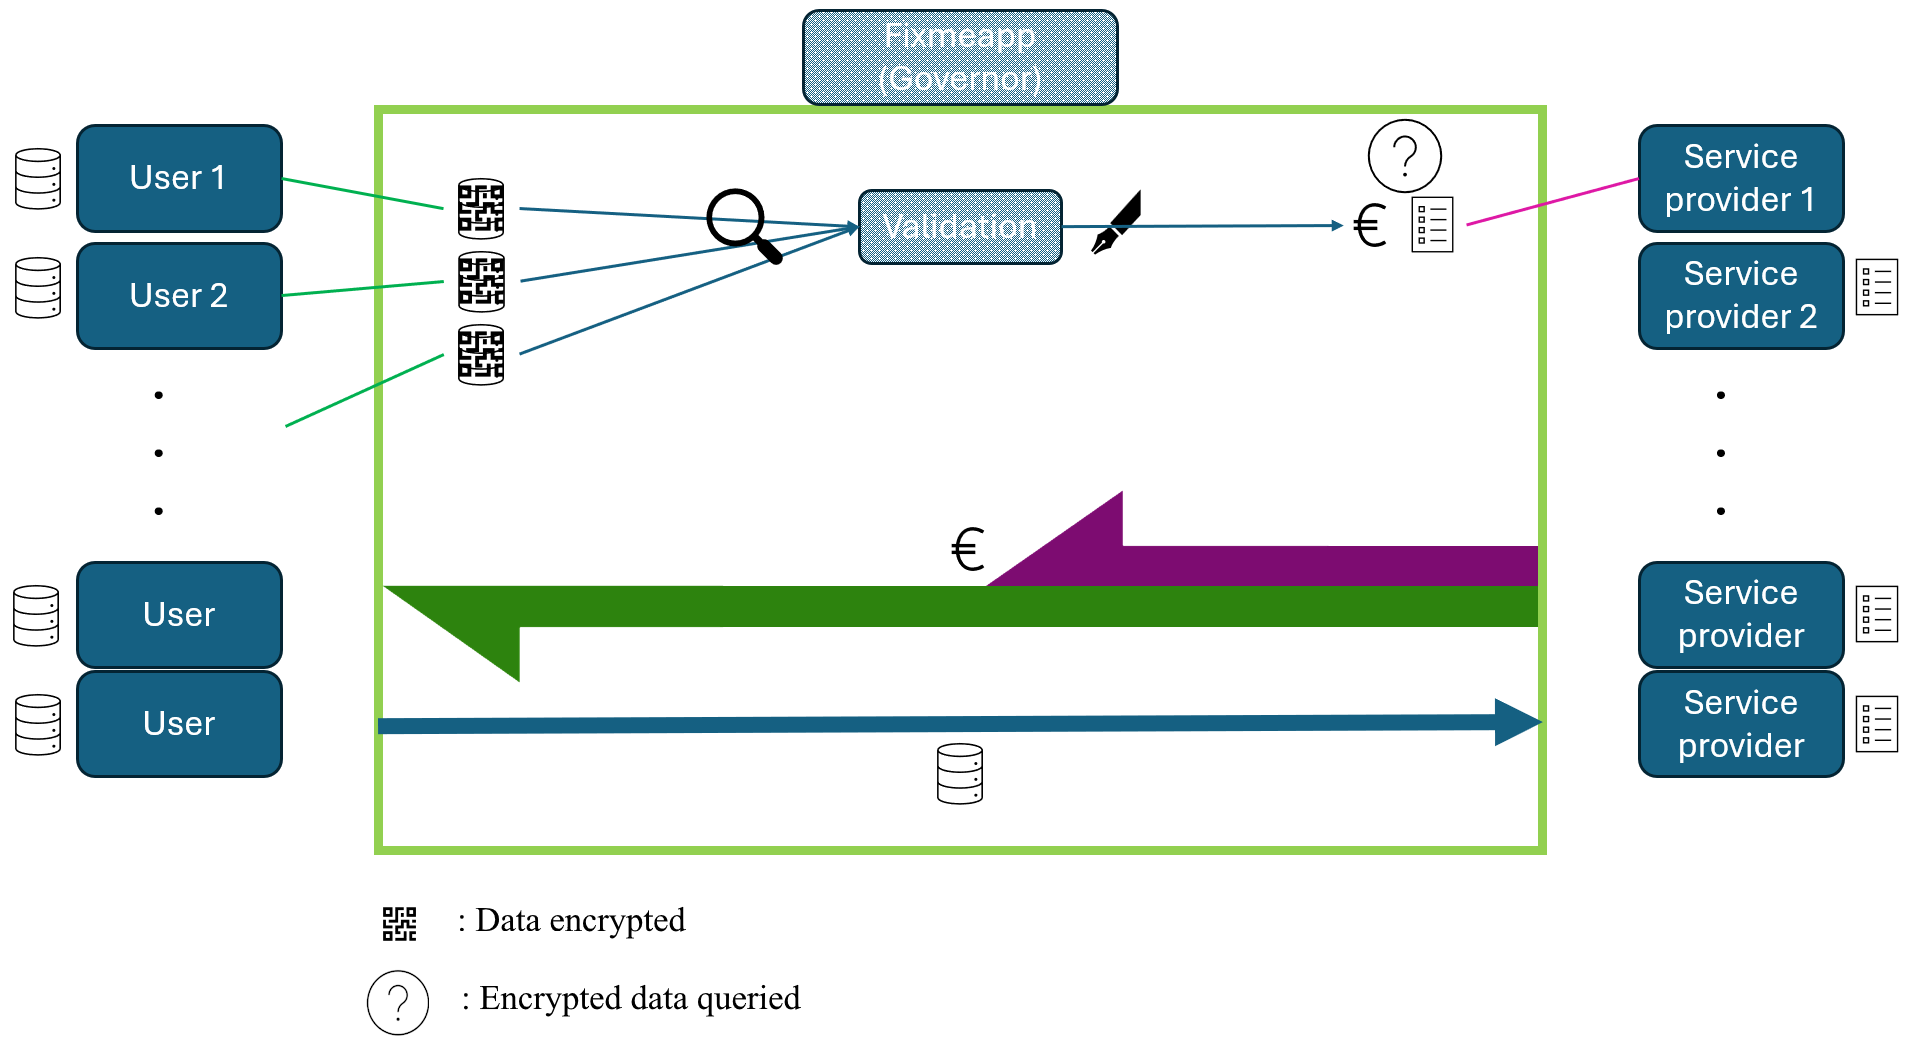
\includegraphics[width=1\linewidth]{images/market_new.png}
    \caption{Fixmeapp's marketplace model, based on the design decisions and business cases in Section 3}
    \label{fig:marketplace_new}
\end{figure}

The data, that the system encodes is the Users'
\begin{itemize}
    \item Geographical polygon,
    \item Demographic data (In this proof of concept: gender and age range),
    \item Booking history (In this case the time of their latest appointment),
    \item Ratings and complaint data,
    \item Allergies
\end{itemize}
Contact data (Name, phone number, e-mail address) are stored in the database for the booking functionality, but not encoded in the Merkle tree structure and cannot be queried by outsiders.
The two programming languages that have a reasonable implementation of the Merkle tree are Python and JavaScript. For the generally better compatibility with any given system and better integration with Fixmeapp's backend, Python is the programming language of choice for this PoC. For generating test data, a python script was used, to simulate a base of 10 000 users.
Considering all aspects of the design and the resources available for the purposes of this thesis, the PoC described in the following subsections was created.

\subsection{Requirements}
One of the goals of this PoC was to make it as universally compatible as possible. This is reflected in its relative self-containment, as the system requires raw data in some tabular form and provides an output in a similar fashion. This is mostly database system independent, leading requirements only in programming packages and some computational power.
The program requires:
\begin{itemize}
    \item Python ver. 3.10+
    \item pymerkle package (ver. 6.1.0)
    \item pandas package (ver. 1.5.1)
    \item numpy package (ver. 1.23.4)
\end{itemize}
Package versions are not the minimum required versions, but the ones used in the creation of the PoC at the time of the writing of this study.
For computations my personal computer was used, with a 11th Gen Intel(R) Cote(TM) i3-1115G4 @ 3.00GHz processor and 8 GBs of RAM. The runtimes should be considered accordingly.

\subsection{Data generation}
It is neither reasonable nor in the spirit of the study to use real user data for the proof of concept. This means test data has to be generated in order for the system to be properly tested. For this I used the script found in section \ref{code:datagen}. The following bash command was used to generate the data:
\begin{verbatim}
    python3 ./generate_table_csv_data.py 
    --output-dir "generated_table_data" 
    --rows-per-table 10000 
    --seed 69
\end{verbatim}
The output was saved in the file ./generated\_table\_data/users.csv in the repository. A snippet of it can be seen on Figure \ref{fig:data_gen_output}. \\
\begin{figure}[H]
    \centering
    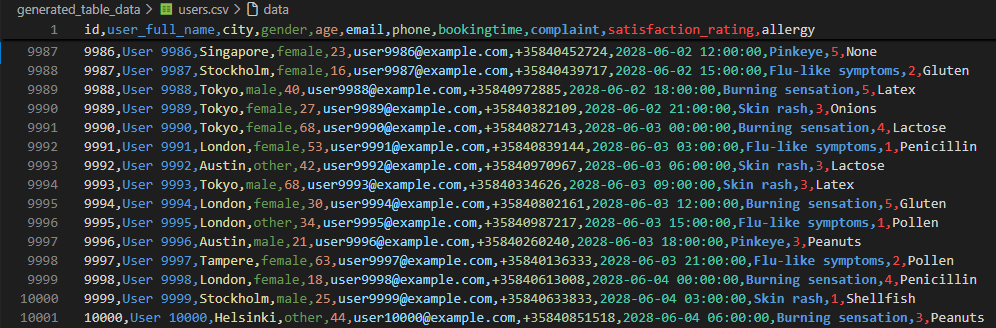
\includegraphics[width=1\linewidth]{images/data_gen_output.png}
    \caption{Snippet of the generated data for 10000 users, random seed used: 69}
    \label{fig:data_gen_output}
\end{figure}


\subsection{Proof of concept}
For better showcasing the proof of concept was written in a jupyter notebook, named merkel\_encoder\_PoC.ipynb. The first step is to read the generated user data, I used pandas for that. Output can be seen in Figure \ref{fig:output_1}.
\begin{figure}[H]
    \centering
    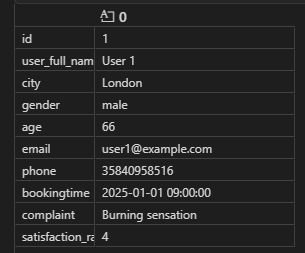
\includegraphics[width=0.8\linewidth]{images/output_1.png}
    \caption{First row of the Dataframe, the first user}
    \label{fig:output_1}
\end{figure}
This data is not completely representative of an actual user base, but it has characteristics that mimic real data sufficiently enough:
The user ids are unique, incrementing numbers. The names are made up of a first name : "User" and a Family name: [incrementing number]. E-mail address is based on the users full name. City is randomly chosen of a list of cities, similarly to complaint and allergies. Age is a random integer between 16-85 and rating is a random integer between 1-5 (stars). The time of the latest booking is probably the least realistic, as it is an incrementing date, starting from 2025 January 1st at 9:00 and incremented by 3 hours every row. Gender is chosen at random from the free options of "other","female" and "male". Phone number is a prefix and a random six digit number after that.\\

Next step is the pseudo-anonymization of the data. In this proof of concept I used two, primitive case-matching bucketing functions for bucketing age into age ranges and cities into geographical polygons. These will be used by the class FixmeTree \ref{code:FixmeTree}, in a static method of the class that will process the entries, and then removes information fit for personal identification (Name, e-mail, phone, age, city). Notably it leaves us with 8 columns ('gender', 'bookingtime', 'complaint', 'satisfaction\_rating', 'allergy', 'age\_range', 'geopolygon' and most importantly user id), allowing for retracing contribution with the unique user id. To best showcase how this works, it is best to take a small-scale example.  Figure \ref{fig:output_2} shows how pseudo-anonymization changes the user data seen in \ref{fig:output_1}, that we will work with for now.
\begin{figure}[H]
    \centering
    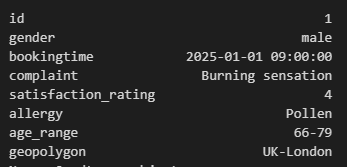
\includegraphics[width=0.8\linewidth]{images/output_2.png}
    \caption{Data entry after pseudo-anonymization}
    \label{fig:output_2}
\end{figure}
Now that the data has been pseudo-anonymised, it is time to encode it in a Merkle tree. For this we will use the FixmeTree class, initialized with the hashing algorithm of 'SHA256'. We chose this, as it seems to be standard algorithm in relevant literature (\cite{liu2021merkle}\cite{papamanthou2024reckle}\cite{zhu2021improved}), for its relatively cheap computing cost.
The tree initialization and encoding looks like the following in code:\label{answer:rq2}
\begin{verbatim}
    tree_medium = FixmeTree(algorithm='sha256')
    data = FixmeTree.preprocess_entry(df.iloc[0])
    for i in range(len(data)):
   tree_medium.append_entry(data.iloc[i])

    print(f'tree size: {tree_medium.get_size()}')
    print(f'tree state: {tree_medium.get_state().hex()}')
\end{verbatim}
One can see, that this package implements Merkle trees in a way, that every attribute needs to be added to the tree one-by-one as leaves. This implementation of the tree is a binary tree, so having 8 ($2^3$) attributes utilizes resources well. The output is a tree with 8 leaves, 3 levels and a root hash of
\begin{verbatim}
5908decf242bb29d443cb6ccfec1c6a65ae867af160915f274c0f43b7bc7bd2f    
\end{verbatim}
as can be seen in Figure \ref{fig:output_2.5}.
\begin{figure}
    \centering
    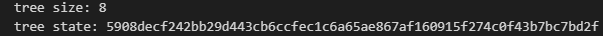
\includegraphics[width=1\linewidth]{images/output_2.5.png}
    \caption{Merkle tree encoding of the first entry}
    \label{fig:output_2.5}
\end{figure}

That concludes setting up the Merkle tree structure, querying method is next:\\
\noindent First, a proof needs to be generated, that something is included on a certain leaf / leaf position on the tree (that is size 8 in our case). In this example we will use position 2, that is gender. We also need a root hash, that we have from the previous code snippet. The base is going to be the information that we want to know it is included. For this, ideally, just hashing the information would be enough, but there is some difference between the implementation of the package and the documentation, so in this case we need to use a one-leaf tree for encoding the query. Implementation of this can be found under \ref{code:verification}. A successful verification returns None (NoneType object in python representing no value), that can be seen in this example with querying for 'male' on leaf 2. But upon querying the same leaf for 'female' or 'other' we get an "InvalidProof: Base hash does not match" error, signaling that the leaf on position 2 in the Merkle tree and the query leaf does not match. (In reality this method checks if their hashes are matching, but if they are hashed with the same algorithm and salting, that they are here, they should have the same hash if they are the same information.) This concludes the small-scale example.\\

The large scale example will take the whole dataset. Building a huge binary tree of $10000 * 8 = 80000$ leaves, meaning a 17 levels deep tree, queried down to the leaves for each of the 10000 users. That is computationally way too expensive compared to building 10000 trees, that are 3 levels deep. For this I chose to go with the latter. Source code for the implementation can be found in Section \ref{code:large_examp}.
It uses a for loop to run the leaf-appending mechanism that could be seen in the small example. The more interesting part is that for querying we need the whole tree object, so all created trees are stored in a pandas DataFrame. This took 10.4 s of computational time, meaning ~1 s per 1000 trees. This includes displaying the results, on the hardware specifications laid out at the beginning of this section. The results can be seen in Figure \ref{fig:output_3}.
\begin{figure}
    \centering
    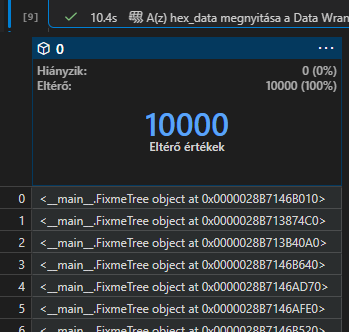
\includegraphics[width=0.9\linewidth]{images/large_encoding_output.png}
    \caption{Large-scale example encoding output. Translation for the values: 'Missing: 0(0\%); Unique: 10000(100\%)}
    \label{fig:output_3}
\end{figure}
Now this database of Merkle tree structures is ready to be queried. Our example query is going to look for users living in the London area in the UK, meaning their geopolygon is 'UK-London'. This is done by extending the small scale example's inclusion verification to larger datasets. This will be done using the test\_geolocation\_match method (implementation found under \ref{code:large_verif}).
For every user, it attempts to verify the proof on the given attribute and criteria to match. If there is None returned, it appends that row, otherwise, we will get an InvalidProof exception, on which the search can just continue. The output is a list of indices, that can be used to query the actual data from the database holding the unencrypted data. The call
\begin{verbatim}
    london_users_lists = test_geolocation_match(hex_data, 'UK-London', 8)
    london_users = df.iloc[london_users_lists]
\end{verbatim}
returns 1209 matching rows in ~0.9 s (Figure \ref{fig:output_4}). That is the time for inclusion verifying 10000 trees and retrieving the matching indices from a different data frame. 
\begin{figure}[H]
    \centering
    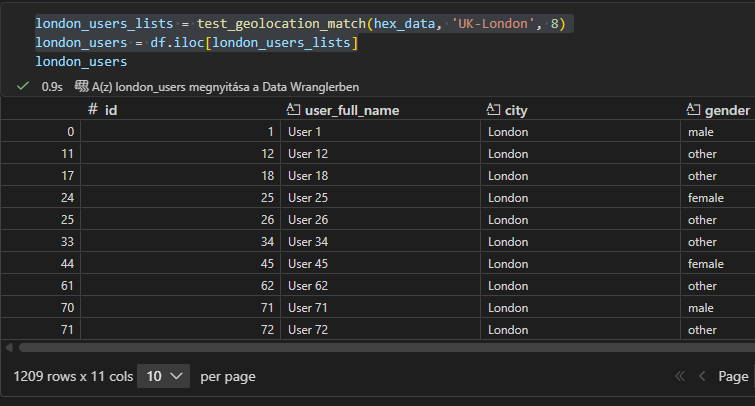
\includegraphics[width=0.9\linewidth]{images/london_match_output.png}
    \caption{Output of the large scale inclusion matching}
    \label{fig:output_4}
\end{figure}
Important to note, that here the matching returns only the row id and the original data is returned based on that. with generated unique user ids this process would be a bit more complicated, as it is not simple row-matching, but should run at a similar speed. 


\clearpage

\section{Discussion and conclusions}
\label{sec:summary}
\subsection{Discussion}
The goal of this thesis was to create a contribution system for an ethical data market that:
\begin{itemize}
    \item That can achieve 
    \begin{itemize}
        \item A Gini coefficient of $G < 0.5$
        \item Relatively high accuracy: $\hat{\pi}^{(k)}_{jl} \leq 1 \text{ , } \forall k$ and some criteria $j$
        \item Relatively high confidentiality: $\epsilon < 5$
        \item Portability of $0.4$ or higher
        \item Effectiveness $\mathcal{E} > 0.5$
    \end{itemize} [RQ 1r \ref{RQ1r}], 
    \item Has a 2-step data collection and criterion matching process that allows for creation of an ethical data economy model [RQ 2 \ref{RQ2}],
    \item Generates some sort of proof that allows for the user account to be identified, even after encoding the data, for them to be rewarded for their contribution [RQ 3 \ref{RQ3}].
\end{itemize}
The analysis of the fulfillment of these criteria will not be in this order, but rather \textbf{RQ 2}, \textbf{RQ 3} and finally \textbf{RQ 1r}, as that requires a longer discussion.\\
Research question two was partially achieved. The PoC reads the raw data, pseudo-anonymises it (step 1) and encodes it in a Merkle tree (step 2), as can be seen in the code snippet \ref{answer:rq2}. It has a criterion matching capabilities, showcased on Figure \ref{fig:output_4}, implemented in \ref{code:large_verif}. For achieving a protocol that is in a similar vein to wibson protocol a contribution system in itself is simply not enough. It needs to be connected to a data marketplace, so there could be a reasonable and fair comparison.\\
Research question three can be answered based on what the PoC is capable of. A proof of inclusion or not inclusion can be generated for any tree and any leaf on said tree. This allows for criteria matching, giving a list of trees. These can then be queried for the user id, giving a way to retrace the original user as a Governor in the system.\\
Research question one is the most extensive one. Due to the limited scope of the thesis it can only be partially answered in a way that one would deem satisfactory.
\begin{itemize}
    \item Fairness: the fairness measure chosen was discrete the Gini coefficient, that is calculated in this case from contribution. As this system could not be properly tested with a good amount of users and transactions, we can only calculate the Gini coefficient for the example. Let's suppose the reward is 1 unit per contribution, we have $n = 10000$ users, and an average reward of $\frac{1209}{10000}$.
    \begin{equation*}
        G_{\text{FixmeTree}}=\frac{\Sigma^{n}_{i=1}\Sigma^{n}_{i=1}\| x_i-x_j \|}{2n(n-1)\overline{x}} = \frac{\Sigma^{10000}_{i=1}\Sigma^{10000}_{i=1}\| x_i-x_j \|}{2*10000*9999*\frac{1209}{10000}}=\\
        \frac{21256638}{24177582} = 0.87
    \end{equation*}
    This fails $G < 0.5$, failing this metric.
    This is obviously signals inequality as only 1209 of the 10000 population contributed, which means only ~12\% of the population was rewarded and that is indeed unequal. querying any one geopolygon will bring the same results, all of them sitting around 12-13\% of the data. If it were a gender question, there would be ~33.3\% contributions, as the data is generated that way. For this estimation to be realistic it needs real users and real customers. Generating data with a better distribution would not be enough, as contribution is just as dependent on the queries as is it dependent on the data.
    \item Accuracy: For accuracy the chosen metric was expectation maximization of the Buyer side. This would require multiple Buyers, but in the current example we only have one. Values are as follows: $k=1$, as there is only 1 Buyer; $n_{il} = 10000$, as they are trying to match the whole dataset. The calculation goes as follows:
    \begin{equation*}
        \hat{\pi}^{(k)}_{jl} = \frac{\Sigma_i \mathbf{I}_{ij} n^{(k)}_{il}}{\Sigma_l \Sigma_i \mathbf{I}_{ij}n^{(k)}_{il}} = \frac{8791}{1209}
    \end{equation*}
    Which larger than one, making it fail our criteria. This would always be the case however, unless the buyer is looking for something that is true for a majority in the database. With an increasing number of Buyers this will not change, because if they are looking to match the same criteria, they are going to get the same score, if they are matching something different, the criteria changes and cannot be counted towards the previous ones. The accuracy measure for this case seems to have been poorly defined. The Buyer is interested in users data, who is matching a profile. Accuracy should be calculated on the Buyers own goals of the data, or the truthfulness of the data provided by the user. It is unrealistic for this thesis to measure cases e.g. "How many users has actually bought a product the Buyer company advertised them from the customers data we provided". That leaves the second option, having to confirm truthfulness of the data with the users. The data is pseudo-anonymised in a way that is losing minimal information, and there is a way for the Governor entity to confirm validity of the data with the user, but that is sadly out of the scope of this thesis.
    \item Confidentiality: The goal was to achieve a differential privacy $\epsilon < 5$. The problem is, that this is ill-defined for deterministic algorithms, as the goal of differential privacy is to make randomized outputs barely distinguishable from one another\cite{sharma2021differential}. A good privacy or integrity measure for Merkle trees would be hash-root collision probabilities \cite{kuznetsov2024merkle}. In this case that is $\frac{1}{2^{256}}$ for fixed pairs. For randomly chosen pairs, the birthday paradox applies, so in the case of $2^{128} (\approx 3.4 \times 10^{38})$ the chance would be about 50\%, but that is not a realistic user base for any application, so integrity is held up.
    \item Portability: This metric is for universality of the data, meaning it scales inversely with confidentiality. The data encoded in Merkle trees is $P=0$, by default gives no information of the data. However, if the data is deemed interesting enough based on the queries, it is provided in a tabular format, making it structured data, giving $P \geq 0.4$. This being a purchase and privacy protection laws not permitting free distribution, that gives an upper bound of $P\leq0.4$, giving us $P=0.4$, fulfilling our goal.
    \item Effectiveness measures how good the data is at answering questions (e.g. what? who? why?). In our example case, the output to the query of users living in the 'UK-London' area was $n_I=1209$. The posed questions relevant here was only the "where?", meaning all the questions have been answered. This metric is, however, biased in this PoC. There are fixed questions, that can be queried (gender, last booking time, complaint, satisfaction rating, allergy, age range, geographical polygon), for which the answer will always have effectiveness score 1. Other information is not stored in the Merkle trees, so there is no queryable information there, thus effectiveness metric, as defined in the research question cannot be realized. For where it is sensible, the effectiveness goal is fulfilled by the PoC.
\end{itemize}
The example showcased in the PoC did not fulfill the fairness, accuracy and confidentiality as defined. It did fulfill confidentiality goals defined for hash tree systems, which it is, portability and effectiveness goals, making it a partial success.\\
This result leaves a lot to be desired. A lot of failures and unmeasurable aspects come from the scope being too small. Only as a working part of an actual data market is it realistic to judge the performance of the system on the FACT principles or other ethical frameworks. This is one, necessary future direction. It would allow for well defined attack surface research and implementation of sufficient counter measure, would allow for realistic data and realistic queries from Buyers, as well as performance metrics computationally.\\
Additional future direction is to connect this system with a running database (for example postgreSQL), testing data reading and identifying users based on uniquely generated user ids. A good addition to this would be to refresh the user database every 30 days and add a cancellation/consent withdrawal policy for transactions. For a more nuanced Buyer query experience implementing query logic to these Merkle trees would be a good next step. For a more nuanced User experience a future implementation of Buyer tracking and consenting for transactions is a good direction. For datasets with large attribute counts, redefining the Merkle tree structure used here to be n-ary trees instead of binary may give a way to speed up querying, at a cost of increasing building time for them.
\subsection{Conclusion}
In this thesis a PoC was created for a Merkle tree-based, privacy preserving contribution system that is designed to be part of an ethical data market model. For that we posed three research questions, analyzed three possible business scenarios and the data relevant to those, to create a design that works best in fulfilling all of the above. The resulting system was implemented in python, using the pymerkle library, fulfilling the business requirements, answering RQ 2 and 3 and partially fulfilling requirements posed in RQ 1, partially answering it. While the PoC can be deemed mostly successful, for a real evaluation further research and testing in a data market environment is required.

\clearpage

%% Bibliography/ list of references
%%
%\thesisbibliography

\bibliography{bibexample} % just insert the bib file name, without .bib, it has to be in the same folder as the .tex file, 
%%%%%%%%%%%%%% separate the bib files with a comma inside the parenthesis
\bibliographystyle{alpha}

\thesisappendix
\section{Thesis repository}
The whole repository can be found in GitHub: \href{https://github.com/balintpragai/elte_aalto_thesis}{Repository}
\section{Data generator script}\label{code:datagen}
\begin{verbatim}
import argparse
import csv
import random
from dataclasses import dataclass
from datetime import datetime, timedelta
from pathlib import Path

@dataclass
class Column:
    name: str
    column_type: str

@dataclass
class TableDefinition:
    name: str
    columns: list[Column]


def fake_city(rng: random.Random) -> str:
    return rng.choice(
        [
            "Helsinki",
            "Tampere",
            "Stockholm",
            "Berlin",
            "London",
            "Austin",
            "Tokyo",
            "Singapore",
        ]
    )


def fake_complaint(rng: random.Random) -> str:
    return rng.choice(
        [
            "Headache",
            "Burning sensation",
            "Flu-like symptoms",
            "Skin rash",
            "Pinkeye",
        ]
    )


def fake_allergy(rng: random.Random) -> str:
    return rng.choice(
        [
            "None",
            "Peanuts",
            "Pollen",
            "Lactose",
            "Penicillin",
            "Dust",
            "Shellfish",
            "Latex",
            "Onions",
            "Gluten",
        ]
    )


def infer_value(
    column_name: str,
    column_type: str,
    row_index: int,
    rng: random.Random,
) -> str | int:
    lower_name = column_name.lower()
    lower_type = column_type.lower()

    if "serial" in lower_type:
        return row_index + 1

    if "integer" in lower_type or "int" in lower_type:
        if "age" in lower_name:
            return rng.randint(16, 85)
        if "rating" in lower_name:
            return rng.randint(1, 5)
        return rng.randint(1, 10_000)

    if "timestamp" in lower_type or "date" in lower_type:
        base = datetime(2025, 1, 1, 9, 0, 0) + timedelta(hours=row_index * 3)
        return base.isoformat(sep=" ")

    if "bookingtime" in lower_name:
        base = datetime(2025, 1, 1, 9, 0, 0) + timedelta(hours=row_index * 2)
        return base.isoformat(sep=" ")
    if "full_name" in lower_name:
        return f"User {row_index + 1}"
    if "city" in lower_name:
        return fake_city(rng)
    if "gender" in lower_name:
        return rng.choice(["male", "female", "other"])
    if "email" in lower_name:
        return f"user{row_index + 1}@example.com"
    if "phone" in lower_name:
        return f"+35840{rng.randint(100000, 999999)}"
    if "complaint" in lower_name:
        return fake_complaint(rng)
    if "allergy" in lower_name:
        return fake_allergy(rng)

    if "text" in lower_type:
        return f"{column_name}_{row_index + 1}"
    if "character varying" in lower_type or "varchar" in lower_type:
        return f"{column_name}_{row_index + 1}"

    return f"value_{row_index + 1}"


def write_csv(table: TableDefinition, rows: int, output_dir: Path, seed: int) -> Path:
    rng = random.Random(f"{seed}:{table.name}")
    output_path = output_dir / f"{table.name}.csv"

    with output_path.open("w", newline="", encoding="utf-8") as handle:
        writer = csv.writer(handle)
        headers = [column.name for column in table.columns]
        writer.writerow(headers)

        for i in range(rows):
            writer.writerow(
                [
                    infer_value(column.name, column.column_type, i, rng)
                    for column in table.columns
                ]
            )

    return output_path


def main(table_list: list[TableDefinition]) -> None:
    parser = argparse.ArgumentParser(
        description="Generate synthetic CSV files for merkle encryption."
    )
    parser.add_argument(
        "--output-dir",
        type=Path,
        default=Path("generated_table_data"),
        help="Directory where CSV files will be written.",
    )
    parser.add_argument(
        "--rows-per-table",
        type=int,
        default=50,
        help="Number of synthetic rows to generate for each table.",
    )
    parser.add_argument(
        "--seed",
        type=int,
        default=42,
        help="Random seed for repeatable outputs.",
    )
    args = parser.parse_args()

    if args.rows_per_table < 1:
        raise ValueError("--rows-per-table must be at least 1.")
    
    if table_list is None or len(table_list) == 0:
        raise ValueError("No table definitions provided.")

    args.output_dir.mkdir(parents=True, exist_ok=True)

    for table in tables:
        path = write_csv(table, args.rows_per_table, args.output_dir, args.seed)
        print(f"Wrote {path}")


if __name__ == "__main__":
    tables = [
        TableDefinition(
            name="users",
            columns=[
                Column(name="id", column_type="SERIAL PRIMARY KEY"),
                Column(name="user_full_name", column_type="TEXT"),
                Column(name="city", column_type="TEXT"),
                Column(name="gender", column_type="TEXT"),
                Column(name="age", column_type="INTEGER"),
                Column(name="email", column_type="TEXT"),
                Column(name="phone", column_type="TEXT"),
                Column(name="bookingtime", column_type="TIMESTAMP"),
                Column(name="complaint", column_type="TEXT"),
                Column(name="satisfaction_rating", column_type="INTEGER"),
                Column(name="allergy", column_type="TEXT"),
            ],
        )
    ]
    main(table_list=tables)
\end{verbatim}
\section{FixmeTree class definition}\label{code:FixmeTree}
\begin{verbatim}
from pymerkle import BaseMerkleTree

class FixmeTree(BaseMerkleTree):

    def __init__(self, algorithm='sha256'):
        """
        Storage setup and superclass initialization
        """
        self.hashes = []

        super().__init__(algorithm)

    @staticmethod
    def preprocess_entry(data):
        """
        Preprocesses data entry before encoding
        e.g. {age: 25, city: "Helsinki"} ->
        b'{"age_range": 18-25, "geopolygon": "FI-Uusimaa"}'
        """
        if isinstance(data, pd.Series):
            data = data.copy()
            data['age_range'] = age_bucketer(data['age'])
            data['geopolygon'] = geopolygon_bucketer(data['city'])
            data = data.drop(labels=['user_full_name', 'email', 'phone', //
            'age', 'city'])
            
        return data
    
    def _encode_entry(self, data):
        """
        Prepares data entry for hashing
        """
        proc_data = str(data)
        encoded_data = proc_data.encode('utf-8')
        return encoded_data
        
    def _store_leaf(self, data, digest):
        """
        Stores data hash in a new leaf and returns index
        """
        self.hashes += [digest]

        return len(self.hashes)


    def _get_leaf(self, index):
        """
        Returns the hash stored by the leaf specified
        """
        value = self.hashes[index - 1]

        return value


    def _get_leaves(self, offset, width):
        """
        Returns hashes corresponding to the specified leaf range
        """
        values = self.hashes[offset: offset + width]

        return values


    def _get_size(self):
        """
        Returns the current number of leaves
        """
        return len(self.hashes)
\end{verbatim}
\section{Verification of inclusion}\label{code:verification}
\begin{verbatim}
from pymerkle import verify_inclusion

prove_tree_true = FixmeTree(algorithm='sha256')
prove_tree_true.append_entry('male')

proof = tree_medium.prove_inclusion(2,8)
base = prove_tree_true.get_leaf(1)
root = tree_medium.get_state(8)

verify_inclusion(base, root, proof)
\end{verbatim}
\section{Large scale Merkle tree encoding}\label{code:large_examp}
\begin{verbatim}
encoded_df = []

for i in range(len(df)):
    entry = None
    locals()["user_tree_" + str(i)] = FixmeTree(algorithm='sha256')
    data = FixmeTree.preprocess_entry(df.iloc[i])
    for j in range(len(data)):
        locals()["user_tree_" + str(i)].append_entry(data[j])
    encoded_df.append(locals()["user_tree_" + str(i)])

hex_data = pd.DataFrame(encoded_df)
hex_data
\end{verbatim}
\section{Large-scale example attribute matching}\label{code:large_verif}
\begin{verbatim}
def test_geolocation_match(dataframe:pd.DataFrame, criteria: str, attribute: int):
    from pymerkle import verify_inclusion, InvalidProof
    
    matching_users = []

    query_tree = FixmeTree(algorithm='sha256')
    query_tree.append_entry(criteria)
    base = query_tree.get_leaf(1)

    for i in range(len(dataframe)):
        user_tree = dataframe.iloc[i][0]

        proof = user_tree.prove_inclusion(attribute, 8)
        root = user_tree.get_state(8)

        try:
            verify_inclusion(base, root, proof)
            matching_users.append(i)
        except InvalidProof:
            continue

    return matching_users
\end{verbatim}

\end{document}